%
%   Prof. Dr. Julian Reichwald
%   auf Basis einer Vorlage von Prof. Dr. Jörg Baumgart
%   DHBW Mannheim
%
%
%	ACHTUNG: Für das Erstellen des Literaturverzeichnisses wird das modernere Paket biblatex
%			 in Kombination mit biber verwendet -- nicht mehr das ältere BibTex!
% 			 Bitte stellen Sie ggf. Ihre TeX-Umgebung
% 			 entsprechend ein (z.B. TeXStudio: Einstellungen --> Erzeugen --> Standard Bibliographieprogramm: biber)
%

\documentclass[
	12pt,
	BCOR=5mm,
	DIV=10,
	headinclude=on,	
	footinclude=off,
	parskip=half,
	bibliography=totoc,
	listof=entryprefix,
	toc=listof,
	pointlessnumbers
	]{scrreprt}

%	Konfigurationsdatei einziehen
% !TEX root =  master.tex

%		LANGUAGE SETTINGS AND FONT ENCODING 
%
\usepackage[ngerman]{babel} 	% German language
\usepackage[utf8]{inputenc}
\usepackage[german=quotes]{csquotes} 	% correct quotes using \enquote{}
\usepackage[T1]{fontenc}

\usepackage{tabularx}
\usepackage[dvipsnames,table]{xcolor}
%\usepackage[english]{babel}   % For english language
%\usepackage{csquotes} 	% Richtiges Setzen der Anführungszeichen mit \enquote{}

% 		HYPERREF
%
\usepackage[
	hidelinks=true % keine roten Markierungen bei Links
]{hyperref}

% Zwei eigene Befehle zum Setzen von Autor und Titel. Ausserdem werden die PDF-Informationen richtig gesetzt.
\newcommand{\TitelDerArbeit}[1]{\def\DerTitelDerArbeit{#1}\hypersetup{pdftitle={#1}}}
\newcommand{\AutorDerArbeit}[1]{\def\DerAutorDerArbeit{#1}\hypersetup{pdfauthor={#1}}}
\newcommand{\Firma}[1]{\def\DerNameDerFirma{#1}}
\newcommand{\Kurs}[1]{\def\DieKursbezeichnung{#1}}


% Correct superscripts 
\usepackage{fnpct}




%		CALCULATIONS
%
\usepackage{calc} % Used for extra space below footsepline



%		BIBLIOGRAPHY SETTINGS
%

% Uncomment the next three lines for author-year-style with footnotes (Chicago)
%\usepackage[backend=biber, autocite=footnote, style=authoryear, dashed=false]{biblatex} 	%Use Author-Year-Cites with footnotes


% Uncomment the next line for IEEE-style 
\usepackage[backend=biber, autocite=inline, style=ieee]{biblatex} 	% Use IEEE-Style (e.g. [1])

% Uncomment the next line for alphabetic style 
% \usepackage[backend=biber, autocite=inline, style=alphabetic]{biblatex} 	% Use alphabetic style (e.g. [TGK12])

% Uncomment the next two lines vor Harvard-Style 
%\usepackage[backend=biber, style=apa]{biblatex} 	
%\DeclareLanguageMapping{german}{german-apa}


\DefineBibliographyStrings{ngerman}{  %Change u.a. to et al. (german only!)
	andothers = {{et\,al\adddot}},
}

%%% Uncomment the following lines to support hard URL breaks in bibliography 
%\apptocmd{\UrlBreaks}{\do\f\do\m}{}{}
%\setcounter{biburllcpenalty}{9000}% Kleinbuchstaben
%\setcounter{biburlucpenalty}{9000}% Großbuchstaben

\setcounter{secnumdepth}{3}

\setlength{\bibparsep}{\parskip}		%add some space between biblatex entries in the bibliography
\addbibresource{bibliography.bib}	%Add file bibliography.bib as biblatex resource


%		FOOTNOTES 
%
% Count footnotes over chapters
\usepackage{chngcntr}
\counterwithout{footnote}{chapter}

%	ACRONYMS
%%%
%%% WICHTIG: Installieren Sie das neueste Acronyms-Paket!!!
%%%
\makeatletter
\usepackage[printonlyused]{acronym}
\@ifpackagelater{acronym}{2015/03/20}
  {%
    \renewcommand*{\aclabelfont}[1]{\textbf{\textsf{\acsfont{#1}}}}
  }%
  {%
  }%
\makeatother

%		LISTINGS
\usepackage{listings}	%Format Listings properly
\renewcommand{\lstlistingname}{Quelltext} 
\renewcommand{\lstlistlistingname}{Quelltextverzeichnis}
\lstset{numbers=left,
	numberstyle=\tiny,
	captionpos=b,
	basicstyle=\ttfamily\small}


%		EXTRA PACKAGES
\usepackage{lipsum}    %Blindtext
\usepackage{graphicx} % use various graphics formats
\usepackage[german]{varioref} 	% nicer references \vref
\usepackage{caption}	%better Captions
\usepackage{booktabs} %nicer Tabs
\usepackage{array}
\usepackage{longtable}
%\newcolumntype{P}[1]{>{\raggedright\arraybackslash}p{#1}}


%		ALGORITHMS
\usepackage{algorithm}
\usepackage{algpseudocode}
\renewcommand{\listalgorithmname}{Algorithmenverzeichnis }
\floatname{algorithm}{Algorithmus}


%		FONT SELECTION: Entweder Latin Modern oder Times / Helvetica
\usepackage{lmodern} %Latin modern font
%\usepackage{mathptmx}  %Helvetica / Times New Roman fonts (2 lines)
%\usepackage[scaled=.92]{helvet} %Helvetica / Times New Roman fonts (2 lines)

%		PAGE HEADER / FOOTER
%	    Warning: There are some redefinitions throughout the master.tex-file!  DON'T CHANGE THESE REDEFINITIONS!
\RequirePackage[automark,headsepline,footsepline]{scrlayer-scrpage}
\pagestyle{scrheadings}
\renewcommand*{\pnumfont}{\upshape\sffamily}
\renewcommand*{\headfont}{\upshape\sffamily}
\renewcommand*{\footfont}{\upshape\sffamily}
\renewcommand{\chaptermarkformat}{}
\RedeclareSectionCommand[beforeskip=0pt]{chapter}
\clearscrheadfoot

\ifoot[\rule{0pt}{\ht\strutbox+\dp\strutbox}DHBW Mannheim]{\rule{0pt}{\ht\strutbox+\dp\strutbox}DHBW Mannheim}
\ofoot[\rule{0pt}{\ht\strutbox+\dp\strutbox}\pagemark]{\rule{0pt}{\ht\strutbox+\dp\strutbox}\pagemark}

\ohead{\headmark}


\begin{document}



\TitelDerArbeit{Analyse und Integration einer passwortlosen Authentifizierung im Unternehmenskontext}
\AutorDerArbeit{Luka Tsipitsoudis}
\Firma{Lufthansa Systems GmbH \& Co. KG}
\Kurs{TINF20CS1}

\definecolor{tabdavid}{RGB}{213,229,255}

\begin{titlepage}
    \begin{minipage}{\textwidth}
            \vspace{-2cm}
            \noindent
            
\includegraphics[scale=0.035]{img/Uzletiforditas.hu-Lufthansa.png} 
             \hfill   
             
\includegraphics{img/logo.jpg}
    \end{minipage}
    
    \vspace{2em}
    \sffamily
    \begin{center}
        \textsf{\large{}Duale Hochschule Baden-W\"urttemberg\\[1.5mm] Mannheim}\\[2em]
        \textsf{\textbf{\Large{}Bachelorarbeit}}\\[3mm]
        \vspace{5em}
        \textsf{\textbf{\Large{\DerTitelDerArbeit}}} \\[1.5cm]
        \vspace{5em}
        \textsf{\textbf{Studiengang Cyber Security}\\[3mm]}
        
        \vspace{3em}
    \vfill
    
    \begin{minipage}{\textwidth}
    
    \begin{tabbing}
        Wissenschaftlicher Betreuer: \hspace{0.85cm}\=\kill
        Verfasser: \> \DerAutorDerArbeit \\[1.5mm]
        Matrikelnummer: \> 4110112 \\[1.5mm]
        Kurs: \> \DieKursbezeichnung \\[1.5mm]
        Bearbeitungszeitraum: \> 06.06.2023 -- 29.08.2023\\ [1.5mm]
        Abgabedatum: \> 29.08.2023\\ [1.5mm]
        Betreuer: \> Stefan Köster\\
        % Ausbildungsfirma: \> \DerNameDerFirma  \\[1.5mm]
        % Betrieblicher Betreuer: \> Oliver Grimm \\
    \end{tabbing}
    
    % \vspace{2cm}
    % Unterschrift Betreuer:  \> \_\_\_\_\_\_\_\_\_\_\_\_\_\_\_\_\_\_ 
    \end{minipage}
    
    \end{center}
    
    \end{titlepage}

\pagenumbering{roman} % Römische Seitennummerierung
\normalfont

%--------------------------------
% Verzeichnisse - nicht benötige Verzeichnisse bitte auskommentieren / löschen.
%--------------------------------

% Ehrenwörtliche Erklärung ewerkl.tex einziehen
% !TEX root =  master.tex

\clearpage
\chapter*{Ehrenwörtliche Erklärung}

% Wird die folgende Zeile auskommentiert, erscheint die ehrenwörtliche
% Erklärung im Inhaltsverzeichnis.

% \addcontentsline{toc}{chapter}{Ehrenwörtliche Erklärung}
Ich versichere hiermit, dass ich meine Projektarbeit mit dem Thema: \textit{\DerTitelDerArbeit} selbstständig verfasst und keine anderen als die angegebenen Quellen und Hilfsmittel benutzt habe. Ich versichere zudem, dass die eingereichte elektronische Fassung mit der gedruckten Fassung übereinstimmt.

\vspace{3cm}


\textbf{Ort, Datum} \hfill 

% \input{ewerkl2.tex}

%   Sperrvermerk
% \chapter*{Sperrvermerk}
Der Inhalt dieser Arbeit: 

\textit{\glqq Entwicklung  einer Software zur Entscheidung der richtigen Projekt Methode. Welche Projektmethode passt zu meinem Projekt? \grqq{}}

darf weder als Ganzes noch in Auszügen Personen außerhalb des Prüfungsprozesses und des Evaluationsverfahrens zugänglich gemacht werden, sofern keine anders lautende Genehmigung des Dualen Partners vorliegt. 

[Ende der Sperrfrist: unbegrenzt]

\vspace{3cm}
Ort, Datum

\textbf{Ort, Datum} \hfill \DerAutorDerArbeit

\cleardoublepage



% LTeX: language=de-DE

\chapter*{Abstract}

\vspace{-2em}

\paragraph*{Englisch}
Passwords are considered to be the most common type of authentication. Despite their high establishment, they have a large number of vulnerabilities. For this reason, some passwordless alternatives for authentication have already been developed. One of these alternatives is the FIDO2 standard. It allows users to log in to online services using an authentication device. Frequently used authentication devices are security keys. These are an external piece of hardware that is only in the possession of the user. The FIDO2 standard is based on asymmetric cryptography, which allows authentication to be more secure than password-based authentication. This is especially due to the fact that FIDO2 credentials cannot be guessed and cannot be affected by data leaks or phishing emails. This thesis deals with the factors of security and usability of FIDO2 and with the integration of FIDO2 into Lufthansa Systems GmbH \& Co. KG.

\paragraph*{Deutsch}
Passwörter gelten seit langer Zeit als die gängigste Art der Authentifizierung. Trotz ihrer hohen Etablierung weisen sie eine Vielzahl an Schwachstellen auf. Aus diesem Grund wurden bereits einige passwortlose Alternativen zur Authentifizierung entwickelt. Eine dieser Alternativen ist der FIDO2 Standard. Er bietet Nutzern die Möglichkeit sich mithilfe eines Authentifizierungsgerätes bei Online-Diensten anzumelden. Häufig genutzte Authentifizierungsgeräte sind dabei Security Keys. Bei diesen handelt es sich um eine externe Hardware, welche sich nur im Besitz des Nutzers befindet. Der FIDO2 Standard basiert auf asymmetrischer Kryptografie, was eine Authentifizierung sicherer gestalten kann als eine passwortbasierte Authentifizierung. Dies liegt insbesondere daran, dass sich FIDO2 Zugangsdaten nicht erraten lassen und nicht von Datenlecks oder Phishing E-Mails betroffen seien können. Diese Arbeit beschäftigt sich mit den Faktoren der Sicherheit und Benutzerfreundlichkeit von FIDO2 und mit der Integration von FIDO2 in die Lufthansa Systems GmbH \& Co. KG.

%	Inhaltsverzeichnis
\tableofcontents



%	Abbildungsverzeichnis
\listoffigures

%	Tabellenverzeichnis
\listoftables

%	Listingsverzeichnis
%\lstlistoflistings

% 	Algorithmenverzeichnis
%\listofalgorithms

% 	Abkürzungsverzeichnis (siehe Datei acronyms.tex!)
\clearpage
\chapter*{Abkürzungsverzeichnis}	
\addcontentsline{toc}{chapter}{Abkürzungsverzeichnis}


\begin{acronym}[RDBMS]
	\acro{LSY}{Lufthansa Systems GmbH \& Co. KG}
	\acro{FIDO}{Fast Identity Online}
	\acro{W3C}{World Wide Web Consortium}
	\acro{SFA}{Single-Factor Authentication}
	\acro{MFA}{Multi-Factor Authentication}
	\acro{CTAP2}{Client-to-Authenticator Protocol 2}
	\acro{NFC}{Near Field Communication}
	\acro{ITU-T}{International Telecommunication Union Telecommunication Standardization Sector}
	\acro{MITM}{Man In The Middle}
	\acro{PAKE}{Password Authenticated Key Exchange}
	\acro{EUF-CMA}{Existential Unforgeability under a Chosen Message Attack}
	\acro{PQ}{Post-Quantum}
	\acro{KEM}{Key Encapsulation Mechanism}
	\acro{TLS}{Transport Layer Security}
	\acro{puvProtocol}{PIN/UV Auth Protocol}
	\acro{SUF}{Strongly Unforgeable}
	\acro{UF}{Unforgeable}
	\acro{OTP}{One-Time Password}
	\acro{HOTP}{HMAC-based One-Time Password}
	\acro{TOTP}{Time-based One-Time Password}
	\acro{HMAC}{Hash-based Message Authentication Code}
	\acro{CDS}{Corporate Directory Service}
	\acro{AD}{Active Directory}
	\acro{JWT}{JSON Web Token}
	\acro{SSO}{Single Sign-On}
	\acro{U2F}{Universal Second Factor}
	\acro{IDS}{Intrusion Detection System}
	\acro{DDoS}{Distributed Denial of Service}
\end{acronym}

\ohead{Acronyms} % Neue Header-Definition


%--------------------------------
% Start des Textteils der Arbeit
%--------------------------------
\clearpage
\ihead{\chaptername~\thechapter} % Neue Header-Definition (inner header)
\ohead{\headmark} % Neue Header-Definition (outer header)
\pagenumbering{arabic}  % Arabische Seitenzahlen



\clearpage
\pagenumbering{arabic}
\setcounter{page}{10}
%	Literaturverzeichnis
\clearpage
\ihead{}

\cleardoublepage

\chapter{Einführung}
Diese Arbeit beschäftigt sich mit passwortlosen Authentifizierungsverfahren. Im Folgenden werden zunächst die Problemstellung und das Ziel der Arbeit erläutert. Anschließend wird der Aufbau der Arbeit beschrieben und auf verwandte Arbeiten eingegangen:

\section{Problemstellung \& Ziel der Arbeit} \label{target}
Die Problemstellung dieser Arbeit bezieht sich auf den aktuellen, passwortlosen Ansatz der Authentifizierung im Unternehmenskontext der \ac{LSY}. Trotz ihrer hohen Etablierung und Verbreitung bieten passwortlose Authentifizierungsverfahren nicht nur Vorteile, sondern auch eine hohe Anzahl an Angriffsvektoren. 

Ziel dieser Arbeit ist es daher passwortlose Authentifizierungsverfahren als Alternative genauer zu betrachten. Verschiedene passwortlose Verfahren werden vorgestellt und ihre individuellen Vor- und Nachteile aufgezeigt. Dabei soll ein besonderes Augenmerk auf den Vergleich der Angriffsvektoren von passwortlosen und passwortbasierten Verfahren gelegt werden. Ein besonderer Fokus liegt auf der Analyse von FIDO2 in Kombination mit einem Security Key. Dabei wird analysiert, ob das Verafahren für die \ac{LSY} geeignet ist und welche Anpassungen vorgenommen werden müssen. Betrachtet werden insbesondere die Aspekte der Sicherheit und der Benutzerfreundlichkeit. Der Fokus liegt auf der Frage, ob passwortlose Verfahren eine Alternative darstellen, welche Passwörter gänzlich ersetzen. 

\section{Aufbau der Arbeit}
Die Arbeit gibt zunächst eine Einführung in die verschiedenen Arten der Authentifizierung und stellt eine Verknüpfung zu den Schutzzielen der Informatik her. Anschließend wird die Passwortbasierte Authentifizierung genauer betrachtet. Dabei werden die typischen Schwachstellen und Angriffsvektoren detailiert aufgezeigt und beschrieben. Auf Basis dieser Erkentnisse werden mögliche passwortlose Alternativen vorgstellt. Diese werden kurz beschrieben und ihre Vor- und Nachteile betrachtet. Spezifischer wird auf die Nutzung von Security Keys (Yubikeys) eingegangen. Ein Fokus liegt dabei auf der Recherche zum Thema der Benutzerfreundlichkeit. Anschließend wird das FIDO2-Protokoll detailiert betrachtet. Die unterliegenden Protkollo WebAuthn und CTAP2 werden dargestellt und deren Funktionsweise erläutert. Hierbei wird ebenfalls der Aspekt der Sicherheit analysiert. So sollen die Unterschiede der passwortbasierten und passwortlosen Authentifizierung verdeutlicht werden, insbesondere im Bezug auf die Sicherheit.

Nach der auf Fachliteratur basierenden Ergebnisse wird die aktuelle Lage der \ac{LSY} dargestellt. Der Fokus liegt dabei auf den aktuellen Prozessen der Authentifizierung. Um die Ergebnisse der Fachliteratur mit der Praxis zu vergleichen, wird eine Implementierung von FIDO2 in Kombination mit einem Security Key vorgenommen innerhalb einer Abteilung der \ac{LSY} vorgenommen. Dabei wird betrachtet, ob und wie gut sich FIDO2 in den Unternehmenskontext der \ac{LSY} integrieren lässt. Die vorgenommene Umsetzung wird aufgezeigt und mit den aktuellen Prozessen verglichen.

Um die Benutzerfreundlichkeit besser bewerten zu können wird auf Basis der erarbeiten Ergebnisse der Fachliteratur ein interaktiver Fragebogen erstellt. Dieser wird innerhalb einer Abteilung der \ac{LSY} durchgeführt. Die Ergebnisse werden ausgewertet und mit den Ergebnissen der Fachliteratur verglichen. Ziel ist es dabei eine individuelle Empfehlung für die \ac{LSY} auszusprechen.

Abschließend soll auf Basis der Literaturrecherche und der Auswertung des Fragebogens eine Empfehlung für die \ac{LSY} ausgesprochen werden. Dabei wird die Frage beantwortet, ob passwortlose Authentifizierungsverfahren eine aktuelle Alternative für die \ac{LSY} darstellen.

\section{Referenzierte Arbeiten}

Bestandteil dieser Arbeit ist eine wissenschaftliche Literaturrecherche. Diese wird insbesondere genutzt, um die aktuelle Lage der Forschung zu passwortlosen Authentifizierungsverfahren zu ermitteln. Insbesondere werden Arbeiten zur Thematik der Nutzung und Schwachstellen von Passwörtern und der aktuellen Nutzung von passwortloser Authentifizierung betrachtet. Im Bereich der passwortlosen Authentifizierung werden insbesondere Arbeiten zu FIDO2 und Security Keys detailliert betrachtet. Die Recherche wird mit Hilfe von Google Scholar und der Bibliothek der DHBW Mannheim durchgeführt. Dabei werden zu wichtigen Aspekten dieser Arbeit mehrere Arbeiten betrachtet, um die Ausagen der Arbeiten zu verifizieren. Ebenfalls werden wissenschaftliche Arbeiten und Artikel aufgegriffen, welche sich in der Literatur als Grundlage etabliert haben und häufig zitiert werden. Da es sich bei der passwortlosen Authentifizierung um ein sehr aktuelles Thema handelt, ist eine Verfizierung der Aussagen teilweise nicht detailiiert möglich. Im Folgenden werden die wichtigsten Arbeiten aufgeführt und kritisch reflektiert:

Die Arbeit \cite{boonkrong2012security} beschäftigt sich insbesondere mit den Grundlagen der Sicherheit von Passwörtern un deren Speicherung. Dabei werden die typischen Faktoren der Authentifizierung beschrieben. Diese bieten eine gute Grundlage für die Unterscheidung von passwortbasierten und passwortlosen Verfahren sowie von \ac{MFA} und \ac{SFA}. 

Für eine Einführung wird die Arbeit \cite{samonas2014cia} genutzt. Diese ist eine häufig zitierte Arbeit, welche sich mit den Schutzzielen der Informatik und deren Entwicklung beschäftigt. Hier werden lediglich die Grundlagen der Schutzziele aus der Arbeit entnommen. Die Arbeit kann allerdings auch für einen tieferen Einblick genutzt werden.

Die Arbeit \cite{chanda2016password} beschäftigt sich insbesondere mit der Speicherung von Passwörtern und den benötigten Aufwand diese zu brechen. Für die durchgeführten Tests, Passwörter zu brechen werden u.a. fünf und sechs stellige Passwörter verwendet. Diese sind in der Praxis nicht relevant, weil eine Passwörter eine höhere Länge aufweisen sollten. Dennoch wird der signifikante Zeitunterschied durch den simplen Unterschied der Passwortlänge deutlich. Auch die Betrachtung einer Veränderung des Zeichenraumes und der Passwortlänge wird betrachtet, welches eine wichtige Erkenntnis für die Sicherheit von Passwörtern darstellt.

Die Arbeit \cite{ives2004domino} betrachtet den Domino-Effekt, welcher bei einer mehrfachen Verwendung eines Passwortes entstehen kann. Dies spielt eine große Rolle für die Sicherheit von Passwörtern und ist ein wichtiger Aspekt für die Betrachtung von passwortlosen Verfahren. Auch wenn das Paper bereits 2004 veröffentlicht wurde, ist der Domino-Effekt auch heute noch relevant und wird von vielen wissenschaftlichen Arbeiten zitiert.

Das Paper \cite{yildirim2019encouraging} beschäftigt sich mit Richtlinien für die Erstellung von Passwörtern. Für diese Arbeit wird lediglich die Erkenntnis des Papers genutzt, dass Richtlinien zu Erstellung von Passwörtern einen kontraproduktiven Effekt haben können. Für einen detailiertere Betrachtung von Maßnahmen, um Passwörter sicherer zu gestalten empfiehlt sich ein Blick in das Paper. Es handelt sich ebenfalls um ein häufig zitiertes Paper.

Für die Einführung der passwortlosen Verfahren werden insbesondere die Arbeiten \cite{chowhan2019password} und \cite{parmar2022comprehensive} genutzt. Diese stellen einige passwortlose Verfahren vor und beschreiben deren Funktionsweise. Beide Arbeiten eignen sich für einen Einblick in weitere Alternativen zur passwortbasierten Authentifizierung. Für eine detailierte Betrachtung der einzelnen passwortlosen Verfahren werden jedoch weitere Arbeiten benötigt.

Für eine Einführung in die Nutzung von Security Key und speziell YubiKeys wird das Datenblatt \cite{yuibkey2023fido2} genutzt. Dabei handelt es sich nicht um eine wissenschaftliche Arbeit, sondern ein Datenblatt des Herstellers Yubico. Dieses Datenblatt wird allerdings lediglich genutzt, um die Funktionen des YubiKeys aufzuführen. Es werden keine Aussagen über die Sicherheit oder die Benutzerfreundlichkeit aus dem Datenblatt übernommen.

Für die Betrachtung der Benutzerfreundlichkeit von Security Keys werden insbesondere die Ergebnisse der Arbeiten \cite{farke2020you}, \cite{lyastani2020fido2} und \cite{reynolds2018tale} genutzt. Es handelt sich dabei um Arbeiten, welche in verschiedenen Umfängen die Benutzerfreundlichkeit von Security Keys untersuchen, indem sie Nutzer befragen und Testphasen durchführen. Diese Erggebnisse werden in dieser Arbeit zusammengeführt, um eine die Benutzerfreundlichkeit von Security Keys zu bewerten. Ebenfalls dienen die Ergebnisse als Grundlage für die Erstellung des Fragebogens dieser Arbeit. So erfolgt eine wissenschaftliche Begründung für die Auswahl der Fragen und ermöglicht es ebenfalls die Ergebnisse der Arbeiten mit den Ergebnissen dieser Arbeit zu vergleichen. Bei der Arbeit \cite{reynolds2018tale} handelt es sich ebenfalls um eine etablierte Arbeit, welche auch in \cite{lyastani2020fido2} aufgeführt wird. 

Für die Betrachtung und Analyse der Funktionsweise von FIDO2 werden ebenfalls die Arbeiten \cite{farke2020you} und \cite{lyastani2020fido2} genutzt. Der Großteil zur detaillierten Funktionsweise von WebAuthn und CTAP2/CTAP2.1 wird allerdings aus den Arbeiten \cite{barbosa2021provable} und \cite{bindel2022fido2} entnommen. Es handelt sich dabei um sehr aktuelle Arbeiten mit einem hohen wissenschaftlichen Anspruch. Die beiden Arbeiten sind die Grundsteine für die Analyse der Sicherheit von FIDO2. Bei \cite{bindel2022fido2} handelt es sich zudem um eine eine Arbeit, welche Teilweise auf den Ergebnissen von \cite{barbosa2021provable} aufbaut.

Für eine wirtschaftliche Einschätzung der Kosten einer ausgenutzten Schwachstelle in Unternehmen wird \cite{databreach} verwendet. Dabei handelt es sich um eine Studie, welche die Kosten von Datenlecks in Unternehmen untersucht. Diese wird allerdings von IBM in Auftrag gegeben und kann daher nicht als komplett unabhängig betrachtet werden. Es handelt sich aber bei dem jährlich veröffentlichten Bericht um eine etablierte Studie, welche häufig in der Fachliteratur aufegegriffen wird. Da in dieser Arbeit allerdings nur ein kurzer Abschnitt auf die wirtschaftlichen Aspekte eingeht wird die Studie als Richtwert verwendet. Für eine detailliertere Betrachtung der wirtschaftlichen Aspekte empfiehlt sich eine weitreichendere Recherche.

Da es sich bei dem Thema Passkeys um eine sehr aktuelle Technologie handelt, ist eine wissenschaftliche Recherche nur teilweise möglich. Da diese Arbeit lediglich einen Ausblick zum Thema Passkeys gibt, wird der Artikel \cite{usecasfido} zur Erklärung der Funktionsweise. Zum aktuellen Stand der Technologie werden die Dokumentationen von Apple \cite{passkeysapple} und Google \cite{passkeysgoogle} \cite{passkeysgoogledev} verwendet.

\chapter{Grundlagen}
Im Folgenden werden auf Basis der fachlichen Literaturrechere die benötigten Grundlagen dieser Arbeit beschrieben und dargestellt:

\section{Einführung in cFront}
\textit{cFront} ist eine Anwendung, welche von der Abteilung cGroup Solutions innerhalb der \ac{LSY} entwickelt wird. Es handelt sich bei der Anwendung um ein Tool, welches an Flughafen Terminals eingesetzt wird. 

Es agiert dabei als Interface für mehrere Anwendung und ermöglicht es dem Nutzer, diese Anwendungen zu starten. Welche Anwendungen sichtbar sind, können je nach Kunde individuell konfiguriert werden. 
\begin{figure}[h]
	\centering 
	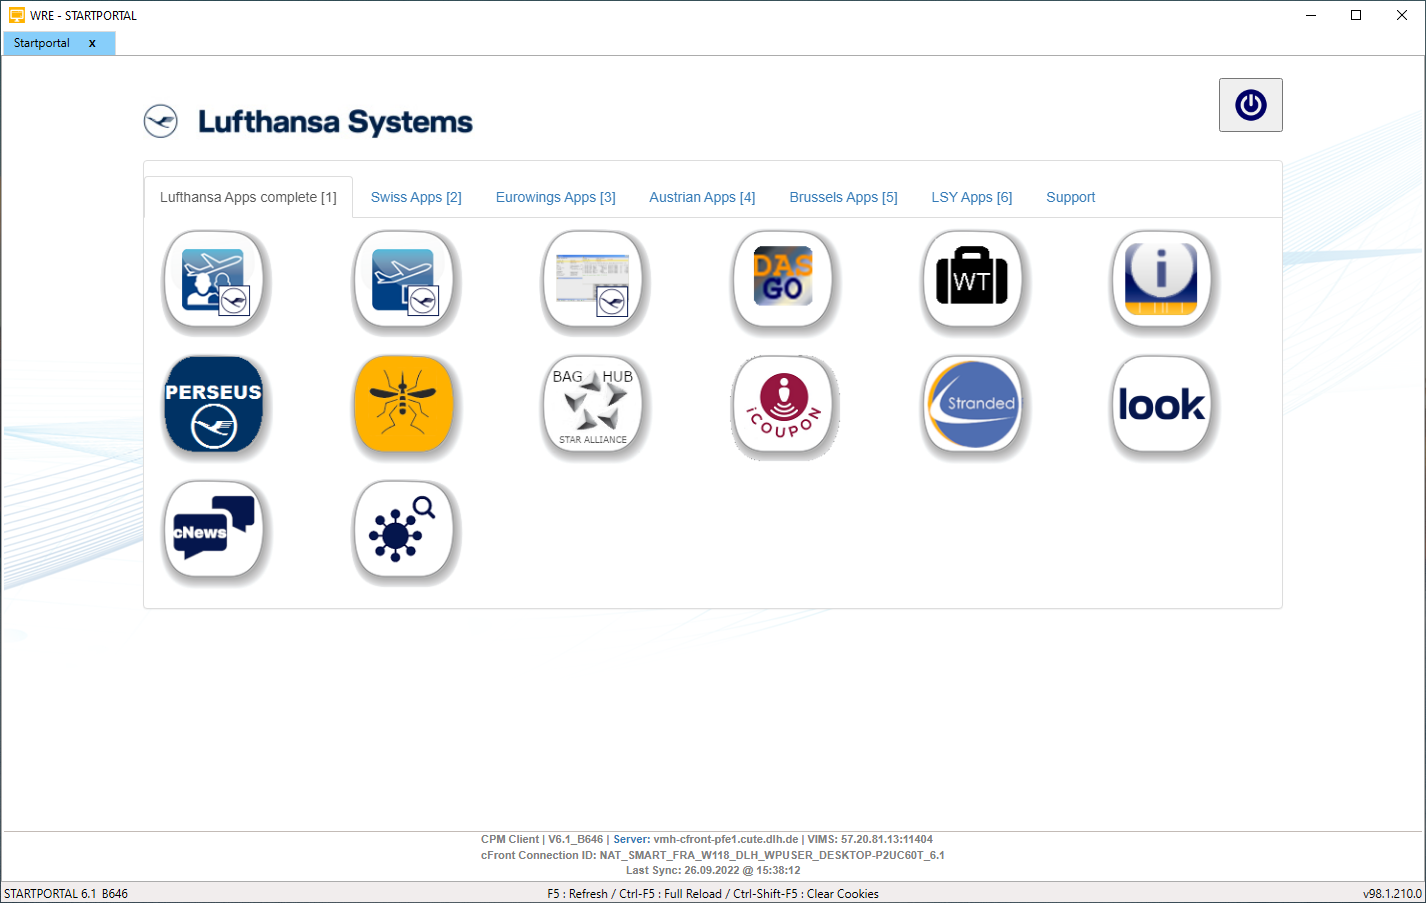
\includegraphics[width=1\textwidth]{img/abbildungen/MicrosoftTeams-image (3).png}
	\captionsetup{format=hang}
	\caption{Umsetzungsmöglichkeit mit Keycloak}
\end{figure}

\section{CIA-Triade}

Die CIA-Triade gehört zu den wichtigsten Darstellungen von Sicherheitszielen innerhalb der Informationssicherheit. Sie beschreibt die drei Schutzziele \textit{Confidentiality} (Vertraulichkeit), \textit{Integrity} (Integrität) und \textit{Availability} (Verfügbarkeit). Im Folgenden werden diese kurz beschrieben:

\begin{figure}[h]
	\centering 
	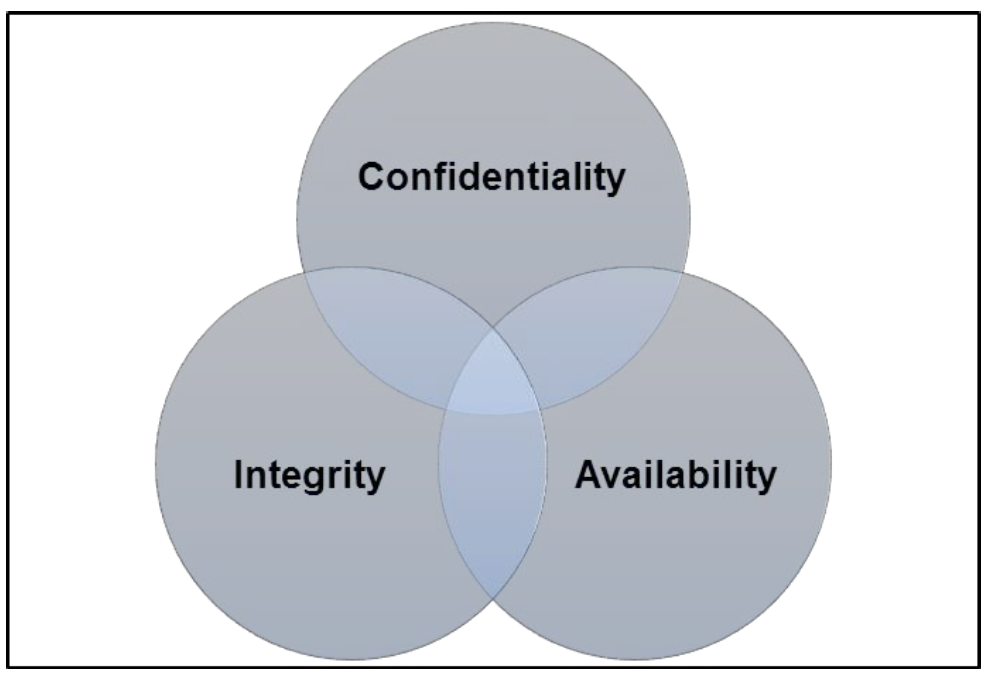
\includegraphics[width=0.5
    \textwidth]{img/abbildungen/CIA-Triad.png}
	\captionsetup{format=hang}
	\caption{CIA-Triad} \label{CIA-Triad}
\end{figure}

\paragraph*{Confidentiality} 
Die Vertraulichkeit gehört zu den wichtigsten Schutzzielen in der Informationssicherheit \cite{samonas2014cia}. Das Wort \textit{Confedentiality} kommt vom lateinischen Wort \textit{confidere} und bedeutet so viel wie \textit{vertrauen} \cite{pons} \cite{samonas2014cia}. Das Schutzziel besagt, dass Informationen und Daten so geschützt sein müssen, dass diese nur von autorisierten Personen und für autorisierte Zwecke genutzt werden können \cite{samonas2014cia}. 
Dies beinhaltet beispielsweise Einschränkungen des Zugriffs auf Informationen und Daten, um die Privatsspähre und persönliches Eigentum zu schützen \cite{samonas2014cia}. Aber auch Verschlüsselungen, eine sichere Authentifizierung und Sicherheitsprotokolle können zur Gewährleistung der Vertraulichkeit beitragen \cite{agarwal2011security}.
Aufgrund der steigenden Wichtigkeit von wirtschaftlichen Aspekten hat die Vertraulichkeit im Vergleich zu früher an Bedeutung verloren \cite{samonas2014cia}. Häufig werden Schutzziele vernachlässigst, um im Gegenzug eine erhöhte Benutzerfreundlichkeit oder Wirtschaftlichkeit zu erreichen.

\paragraph*{Integrity}  
Das Wort Integrity leitet sich vom lateinischen Wort \textit{tangere} ab und bedeutet so viel wie \textit{berühren} \cite{pons}. Durch die Vorsilbe \textit{In-} soll eine Gegenteilige Bedeutung entstehen im Sinne von \textit{Unberührbarkeit} \cite{samonas2014cia}. 
Die Integrität soll somit garantieren, dass Daten nicht verändert werden können, ohne dass dies bemerkt wird \cite{agarwal2011security}. Schickt ein Sender $S$ beispielsweise eine Nachricht an einen Empfänger $E$, so soll die Nachricht identisch beim Empfänger $E$ ankommen, wie sie vom Sender $S$ gesendet wurde \cite{agarwal2011security}.
Umsetzungsmöglichkeiten die Integrität zu schützen beinhalten Maßnahmen wie beispielsweise das Verwenden einer Firewall, \ac{IDS} oder auch digitale Signaturen \cite{agarwal2011security}.
\paragraph*{Availability}
Das Wort Availability leitet sich vom lateinischen \textit{valere} ab und bedeutet so viel wie \textit{kräftig sein}. Die Verfügbarkeit bezieht sich also auf einen zeitnahen und und zuverlässigen Zugriff auf Informationen und Daten \cite{samonas2014cia}. Zuverlässig bedeutet dabei auch, dass ein Zugriff möglichst ohne Unterbrechungen und unabhängig vom Standort möglich ist \cite{agarwal2011security}.
Verfügbarkeit kann beispielsweise durch Netzwerksicherheit (z.B. Schutz vor \ac{DDoS}) oder Fehlertoleranz (z.B. durch Limitierung von Authentifizierungsversuchen) gewährleistet werden \cite{agarwal2011security}.

Ein wichtiger Aspekt der Schutzziele ist, dass diese nicht unabhängig voneinander betrachtet werden dürfen. Vielmehr handelt es sich, um ein Zusammenspiel der verschiedenen Schutzziele (siehe \ref*{CIA-Triad}). So kann eine Maßnahme beispielsweise mehrer Schutzziele schützen. Ebenfalls lassen sich weitere Schutzziele aus den drei bestehenden ableiten. Häufig werden erweiterte Schutzziele wie beispielsweise Authenticity (Authentizität) oder Non-repudiation (Nicht-Abstreitbarkeit) \cite{samonas2014cia} definiert. Diese können dabei zumeist von einem oder mehreren Schutzzielen der CIA-Triade abgeleitet werden. Die folgende Grafik zeigt beispielhaft einige erweiterte Schutzziele und deren Bezug zu der CIA-Triade:

\begin{figure}[h]
	\centering 
	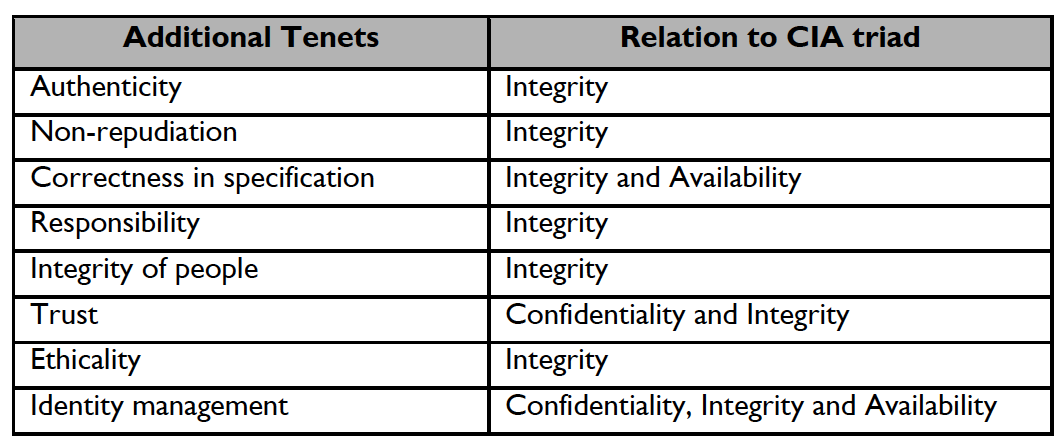
\includegraphics[width=0.8\textwidth]{img/abbildungen/Schutzziele.png}
	\captionsetup{format=hang}
	\caption{Erweiterte Schutzziele} \label{Schutzziele}
\end{figure}


\section{Arten der Authentifizierung}

\begin{figure}[h]
	\centering 
	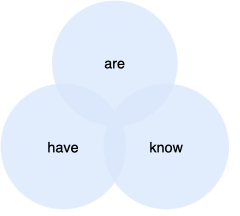
\includegraphics[width=0.4\textwidth]{img/abbildungen/factors.png}
	\captionsetup{format=hang}
	\caption{Faktoren der Authentifizierung}
\end{figure}

Die Authentifizerung dient häufig als erste Verteidigungslinie von Systemen \cite{boonkrong2012security}. Die Authentifizierung gilt als erweitertes Schutzziel und ist eine der wichtigsten Schutznmaßnahmen von Systemen. Sie übernimmt die Kontrolle über die Zugänge von Systemen und bestimmt wer oder was autorisiert ist diese zu nutzen. In der Fachliteratur wird häufig zwischen drei verschiedenen Arten der Authentifizierung unterschieden, welche umgangssprachlich auch als \textit{Faktoren} bekannt sind. Diese sollen im Folgenden beschrieben werden:

\paragraph*{Something you know:}
Die meistgenutzte Art der Authentifizierung basiert auf dem Wissen des Nutzers. Diese Methode nutzt Informationen - welche nur dem Nutzer bekannt sind - und bestätigt somit seine Identität \cite{boonkrong2012security}. Das bekannteste Verfahren ist dabei die Nutzung von Passwörtern, welche nur dem Nutzer bekannt sein sollten. Weitere Verfahren dieser Kategorie wären allerdings auch Sicherheitsfragen. Diese werden initial vom Nutzer beantwortet und im weiteren Verlauf zur Authentifizierung abgefragt.

\paragraph*{Something you have:}
Diese Art der Authentifizierung nutzt physische Objekte, um die Identität des Nutzers zu verifizieren. Es handelt sich um Objekte die sich lediglich im Besitz des Nutzers befinden \cite{boonkrong2012security}. Mögliche Beispiele für diese Methode sind Smartcards, welche an physische Zutrittskontrollen gehalten werden müssen oder Hardware Tokens, die für die Anmeldung an Systemen genutzt werden.

\paragraph*{Something you are:}
Diese Art der Authentifizierung basiert auf der Inhärenz. Das bedeutet, dass zur Verifizierung der Identität des Nutzers biometrische Merkmale verwendet werden \cite{boonkrong2012security}. Dazu gehören u.a. Fingerabdrücke, Geischtserkennung und Iris-Scans. Diese Methode hat sich besonders im Bereich der mobilen Systeme etabliert, so bietet Apple bei seinen Smartphones beispielsweise eine Authentifizierung per Fingerabdruck (\textit{Touch ID}) oder Gesichtserkennung (\textit{Face ID}) an CITE. Aber auch Microsoft bietet mittlerweile eine Authentifizierung mittels biometrischer Daten an (\textit{Windows Hello} und \textit{Hello for Business}) CITE.

Wie schon bei der CIA-Triade lassen sich auch hier weitere Arten ergänzen oder ableiten. Eine weitere Art ist beispielsweise \textbf{something you produce} \cite{boonkrong2012security}. Diese Art der Authentifizierung leitet sich teilweise von dem Faktor \textit{something you are} ab. Sie nutzt beispielsweise die Stimme des Nutzers oder seine (digitale) Unterschrift, um seine Identität zu verifizieren \cite{boonkrong2012security}. 

Die verschiedenen Arten der Authentifizierung spielen auch bei der Unterscheidung zwischen einer \ac{SFA} und einer  \ac{MFA} eine wichtige Rolle. Wird eine einzelner Faktor genutzt, so bezeichnet man dies als \ac{SFA}. Werden mehrere Faktoren genutzt handelt es sich um eine \ac{MFA}.

\section{Passwortbasierte Authentifizierung}\label{pw-auth}

    Die heutzutage am häufigsten genutzte Methode zur Authentifizierung ist die passwortbasierte Authentifizierung \cite{chanda2016password} \cite{boonkrong2012security} \cite{yildirim2019encouraging}. Diese basiert auf dem Faktor \textit{something you know}, also auf dem Wissen der Nutzer. Zumeist handelt es sich um alphanumerische Passwörter, welche aus einer Kombination von Groß- und Kleinbuchstaben, Zahlen und Sonderzeichen bestehen \cite{chanda2016password}. Die Sicherheit informationstechnischer Systeme ist somit abhängig von der Sicherheit der genutzten Passwörter \cite{boonkrong2012security}. Trotz ihrer weitreichenden Verbreitung gelten Passwörter als eine der größten Sicherheitsrisiken für Systeme, da sie vile Schwachstellen und Angriffsvektoren bieten \cite{yildirim2019encouraging} \cite{farke2020you}. Laut einer Studie von \textit{Verizon} basierten 2017 81\% der Hackerangriffe auf der Kompromittierung von Passörtern \cite{barbosa2021provable} \cite{verizon2017}. Eine weitere Studie zeigt auf, dass 2017 Phishing E-Mails die Angriffsmethode darstellte \cite{Symantec} \cite{barbosa2021provable}. Diese sind darauf ausgelegt an Passwörter von Nutzern zu gelangen. Eine Vielzahl von großen Unternehmen wurden bereits Opfer von der Veröffentlichung von Passwörtern, obwohl ein hoher Aufwand betrieben wird, um diese zu schützen \cite{boonkrong2012security}. Da sich die Enthüllung der Passwörter allerdings als Angriffsziel bei Angreifern etabliert hat, ist selbst ein hoher Aufwand nicht mehr immer ausreichend, um jene zu schützen \cite{boonkrong2012security}. Der entstehende Schaden ist immens, da es sich um einen hohen Geldwert, aber u.a. auch um einen Reputationsschaden handeln kann. Trotz der bekannten Schwachstellen und bereits entwickelten alternativen Ansätzen, bleibt das Passwort weiterhin genutzt \cite{ives2004domino}. Dies liegt insbesondere an der Einfachheit und dem geringen Aufwand, welche die Nutzung von Passwörtern mit sich bringt \cite{yildirim2019encouraging}.

    Passwörter können durch verschiedene Arten von Angriffen kompromittiert werden. So können Angreifer beispielsweise Zugriff auf die Datenbank erhalten, in welcher die Passwörter gespeicghert werden, aber auch auf persönlicher Ebene können Passörter erlangt werden. Dabei spielt das sog. Social Engineering eine große Rolle. Durch Shoulder Surfing können Angreifer versuchen Nutzern beim Passwort eintippen zuschauen. Mit Hilfe von Dumpster Diving können beispielsweise aufgeschriebene Passwörter erlangt werden. Zu den häufigsten Social Engineering Angriffen gehören allerdings die bereits beschriebenen Phishing Mails. Auf technischer Ebene ist ebenfalls ein Einsatz von Keyloggern möglich, welche alle Tastendrücke des Nutzers speichert. Ein häufig gewähltes und sehr effektives Mittel bei schlechten Passwörtern sind allerdings Brute-Force- und Dictionary-Angriffe. Diese kompromittieren Passwörter durch das stupide Ausprobieren aller möglichen Kombinationen oder die Nutzung von Tabellen, welche die meistgenutzten Passwörter beinhalten \cite{chanda2016password} \cite{morii2017research}.

    Um Passwörter resistenter gegen Brute-Force-Angriffe zu gestalten, kann eine Erweiterung des Zeichenraums oder der Passwort-Länge genutzt werden. So wird die mögliche Anzahl an Kombinationen des Passworts erhöht. Je mehr mögliche Kombinationen es gibt, desto schwieriger wird es Passwörter durch Erraten zu komprommittieren \cite{chanda2016password}. Wichtig ist hierbei, dass die Erweiterung der Passwortlänge deutlich effektiver ist als die Erweiterung des Zeichenraums. Betrachtet man die Anzahl aller Elemente des Zeichenraums $Z$ und die Passwortlänge $L$, so wird die Komplexität eines Passwortes durch $Z^L$ abgebildet. Während die Erweiterung der Passwortlänge ein exponentielles Wachstum aufweist, steigt bei einer Erweiterung des Zeichenraums die Steigung lediglich linear. Die Effektivität längerer Passwörter wird ebenfalls in \textbf{\ref{EntropyvsLength}} und \textbf{\ref{timetobreak}} dargestellt. \textbf{\ref{EntropyvsLength}} stellt die Entropie von Passwörtern in Abhängigkeit ihrer Länge dar. Dabei werden ebenfalls verschieden große Zeichenräume betrachtet. Es wird deutlich, dass selbst eine hohe Differenz des Zeichenraumes lediglich einen geringen Einfluss auf die Entropie hat. Unabhängig vom Zeichenraum aber dennoch eine hohe Entropie durch ein größere Länge möglich ist. \textbf{\ref{timetobreak}} stellt die benötigte Zeit zum Brechen von Passwörtern in Abhängigkeit zu ihrer Länge dar. Bei beiden Varianten handelt es sich um eine zu kurze Länge eines Passwortes, allerdings ist der signifikante Unterschied durch die Erweiterung der Passwortlänge um eins deutlich erkennbar.

    \begin{figure}[h]
        \centering 
        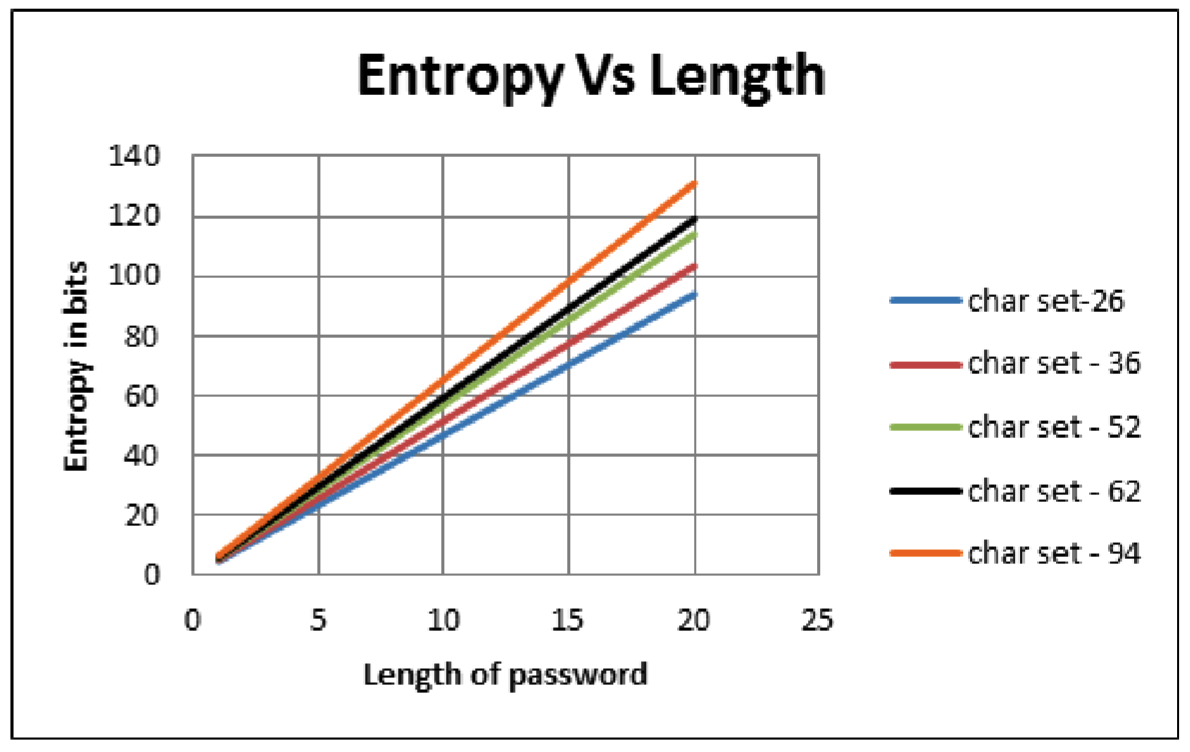
\includegraphics[width=0.7\textwidth]{img/abbildungen/entropy-length.png}
        \captionsetup{format=hang}
        \caption{Entropie in Abhängigkiet der Passwortlänge} \label{EntropyvsLength}
    \end{figure}
    
    \begin{figure}[H]
        \centering 
        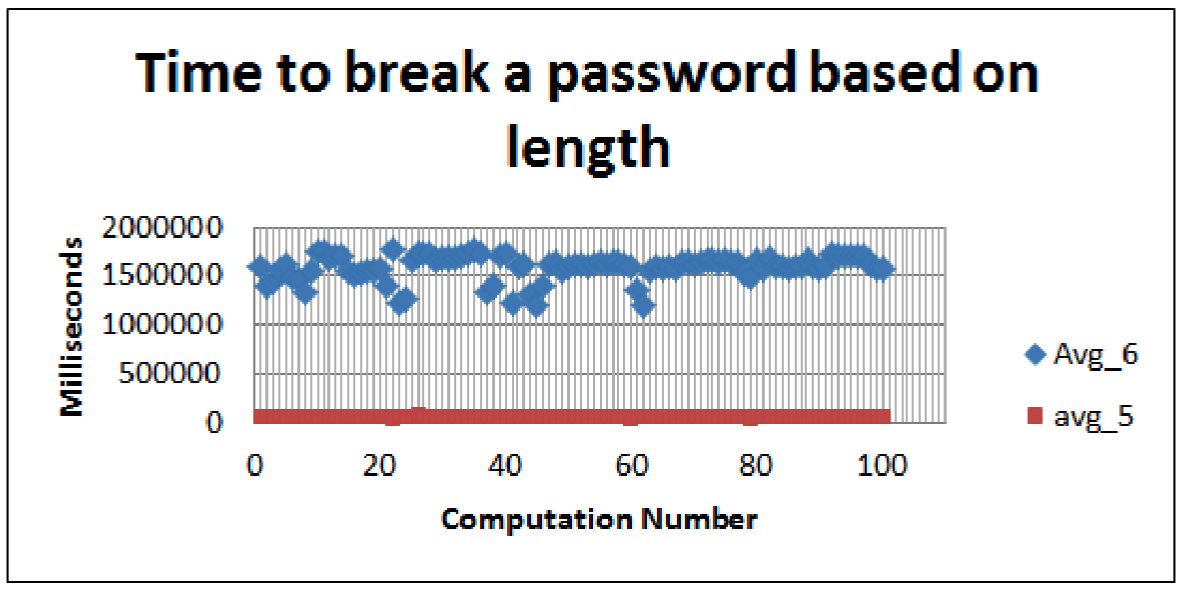
\includegraphics[width=0.7\textwidth]{img/abbildungen/length-time.png}
        \captionsetup{format=hang}
        \caption{Zeit, um ein Passwort zu brechen in Abhängigkeit zu der Länge} \label{timetobreak}
    \end{figure}

    Zwei Angriffsvektoren sind dabei zumeist betroffen: die Speicherung und der Mensch. Im Folgenden soll präziser erläutert werden, was diese beiden Angriffsvektoren so verwundbar machen:

    \textbf{Speicherung:}

    Viele Angreifer versuchen Passwörter zu kompromittieren, indem sie Zugriff auf die Datenbank erhalten, in welcher die Passwörter gespeichert sind. Mit Hilfe der erlangten Passwörtern erhoffen sie sich zumeist einen erweiterbaren Zugriff auf Systeme oder nutzen die Passwörter, um ihre Opfer zu erpressen \cite{boonkrong2012security}. Der wichtigste Faktor für den Erfolg solcher Angriffe spielt die Art der Speicherung. Abhängig von der Art wie Passwörter gespeichert sind offenbaren sich auch verschiedene Schwachstellen \cite{chanda2016password}.
    Die schlechteste, aber dennoch immer noch genutzte Art Passwörter zu speichern ist die Speicherung von Passwörtern im Klartext. Die Passwörter werden also in lesbarer Form gespeichert. Haben Angreifer also Zugriff auf die Datenbank, so können sie alle gespeicherten Passwörter ohne weiteren Aufwand auslesen \cite{chanda2016password}.

    Eine bessere Variante - allerdings weitaus nicht optimale - ist die Verschlüssellung der gespeicherten Passwörter. Der größte Kritikpunkt an dieser Variante ist allerdings, dass Verschlüssellungen zurückführbar sind. Das bedeutet mit dem Besitz des benötigten Schlüssels, lassen sich alle gespeicherten Daten ebenfalls in Klartext umwandeln. Hierbei müssen Angreifer also einen weiteren Aufwand erbringen, um an den benötigten Schlüssel zu gelangen. Sind sie allerdings im Besitz dieses Schlüssels können sie ebenfalls alle gespeicherten Passwörter auslesen \cite*{chanda2016password}. 

    Um die Sepicherung weiter zu optimieren sollte somit keine Zurückführbarkeit bestehen. Dies kann mit Hilfe von Hashing umgesetzt werden. Sog. Hashfunktionen erhalten einen Eingabewert und bilden diesen auf (im Optimalfall) einen einzigen Ausgabewert ab. Dieser Ausgabewert ist nicht zurückführbar auf den Eingabewert. Komprommittieren Angreifer also die Datenbank, in welcher die Passwörter gespeichert sind, können diese die gespeicherten Werte nicht direkt weiterverwenden. Auch dieser Ansatz birgt allerdings Schwachstellen. So lassen sich beispielsweise sog. Rainbow-Tables nutzen, um Hash-Werte zurückzuführen. Dies wird ermöglicht indem häufig genutzte Passwörter gehashed werden und dann mit Hash-Werten innerhalb der Datenbank verglichen werden \cite{chanda2016password}. 

    Um auch diese Schwachstelle zu verhindern, wird ein sog. Salt benötigt. Dabei wird an jedes Passwort, bevor es gehashed wird, ein individueller randomisierter Wert gehangen. Somit wird verhindert, dass sich der gespeicherte Hashwert mit Hilfe von Rainbow-Tables vergleichen lässt. Auch eine Umsetzung mit zwei Salt-Werten ist möglich. Dabei ist ein Salt öffentlich und der andere privat. So kann ebenfalls ein Schutz gegen offline-Angriffe geboten werden \cite{chanda2016password}.

\textbf{Faktor Mensch:}

Neben den aufgezählten technischen Aspekten, stellt der Mensch selbst eine der größten Angriffsvektoren bezogen auf Passwörter dar \cite{ives2004domino} \cite{yildirim2019encouraging}. Eins der größten Problem stellt der Aspekt dar, dass von Menschen erstellte Passwörter keine echten Zufallswerte sind. Das liegt insbesondere daran, dass Nutzer sich ihre Passwörter merken müssen. Je komplexer ein Passwort gestaltet ist, desto schwieriger wird es für Nutzer sich dieses zu merken - insbesonere, wenn sie sich mehrere verschiedene Passwörter merken müssen. Daher beinhalten Passwörter häufig Informationen, welche einen Bezug zum Inhaber haben. Dazu gehören Beispielsweise Namen, Geburtsdaten, Adressen, oder andere persönliche Informationen. Auch Passwörter, welche einfache Muster beinhalten sind sehr beliebt. Dazu gehören beispielsweise \textit{qwertz}, welches die ersten Buchstaben auf der Tastatur darstellt und \textit{123456}. Solche Passwörter können sich Menschen besser einprägen, was notwendig ist, wenn Passwörter häufig genutzt werden müssen. Aus dem identischen Grund neigen Nutzer ebenfalls dazu ein Passwort für mehrere Systeme zu nutzen \cite{chanda2016password} \cite{boonkrong2012security} \cite{yildirim2019encouraging}. 

Die genannten Faktoren führen dazu, dass die Anzahl an genutzten Kombinationen für ein Passwort deutlich geringer ist als die gesamte Menge an möglichen Kombinationen \cite{boonkrong2012security}. Das macht von Menschen erstellte Passwörter deutlich anfälliger für Angriffe, da diese einfacher zu erraten sind \cite{chanda2016password}. Dies liegt häufig auch daran, dass die Motivation der Nutzer häufig gering ist, komplexe Passwörter zu erstellen, weil sie sich der Gefahr von schwachen Passwörtern nicht bewusst sind \cite{yildirim2019encouraging}. Kontraproduktiv wirken in diesem Zusammenhang auch Policies und Richtlinien zur Erstellung von Passwörtern \cite{yildirim2019encouraging}. Sind die Richtlinien zur Erstellung von Passwörtern zu komplex, tendieren Nutzer bewusst dazu Muster in das Passwort einzubauen, um sich dieses zu merken. Dies führt zu einem gegenteiligen Effekt, da die Sicherheit und die Komplexität der Passwörter dadurch sinkt. Die These, dass solche Richtlininien zwangsweise zu einer erhöhten Sicherheit beitragen ist somit ein Irrglaube \cite{yildirim2019encouraging} \cite{morii2017research}.

Ein weiteres Problem stellt die die bereits genannte mehrfache Nutzung eines Passwortes für verschiedene Systeme dar. Aktive Internet-Nutzer verwalten im Durchschnitt 15 Passwörter pro Tag \cite{ives2004domino}. Um sich also das Einprägen verschiedener Passwörter zu ersparen, wählen Nutzer tendenziell lieber ein Passwort. Das führt häufig zu einem Domino-Effekt im Falle einer Passwort-Kompromittierung. Gelangen Angreifer an ein einzelnes Passwort des Nutzers, ist es häufig möglich mit diesem auch Zugriff auf andere Systeme zu gelangen \cite{ives2004domino} \cite{morii2017research}. 


\section{Passwortlose Authentifizierung}

Unter dem Sammelbegriff der passwortlosen Authentifizierung werden verschiedene Verfahren zusammengefasst, welche die Nutzung von Passwörten ersetzen sollen. Im Gegensatz zur passwortbasierten Authentifizierung steht also nicht mehr der Faktor \textit{something you know} im Vordergrund, da das Wissen des Nutzers nicht mehr die Grundlage zur Verifizierung seiner Identität darstellen soll. Die \ac{FIDO} Allianz nutzt den Begriff passwortlose Authentifizierung beispielsweise, um eine eine \ac{SFA} oder \ac{MFA} mit der Hilfe eines Security Keys zu beschreiben \cite{farke2020you}. 

Passwortlose Verfahren werden dabei als sicherer im Vergleich zur passwortbasierten Alternative angesehen, da viele der in \textbf{\ref{pw-auth}} aufgeführten Angriffsvektoren passwortlosen Ansätze nicht existieren \cite{chowhan2019password} \cite{parmar2022comprehensive}. Zudem erhofft man sich eine zusätzliche erhoffte Benutzerfreundlichkeit durch passwortlose Verfahren - insbesondere, weil Nutzer sich keine Passwörter mehr merken müssen und so ein geringerer Aufwand besteht \cite{chowhan2019password}.

Passwortlose Verfahren haben sich jedoch noch nicht flächendeckend durchgesetzt und sind nicht annähernd so weit verbreitet wie die Nutzung von Passwörtern. Dies lässt sich auf mehrere Faktoren zurückführen. Häufig genannte Gründe innerhalb der Fachliteratur sind die Umgewöhnung der Nutzer an eine neuartige Authentifizierung, welches als Hürde zur Etablierung der passwortlosen Verfahren angesehen wird. Aber auch zusätzliche entstehende Kosten durch die Integration der neuen Verfahren können eine Verbereitung ausbremsen \cite{chowhan2019password}. Ein detailierter Einblick in die Vor- und Nachteile in Bezug auf der Benutzerfreundlichkeit wird in \textbf{\ref{Yubikey}} gegeben.

Es gibt dabei eine Vielzahl an Möglichkeiten eine passwortlose AUthentifizierung umzusetzen. Eine der am häufigsten genutzen Varianten ist die Nutzung von Security Keys in Kombination mit FIDO2. Diese liegen im Fokus dieser Arbeit und werden in \textbf{\ref{Yubikey}} und \textbf{\ref{fido2}} genauer beschrieben. Dennoch sollen auch mögliche Alternativen kurz vorgestellt werden:


\begin{figure}[h]
	\centering 
	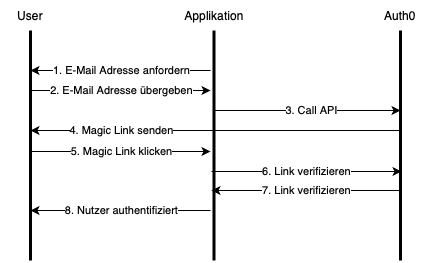
\includegraphics[width=0.7\textwidth]{img/abbildungen/magic_link.png}
	\captionsetup{format=hang}
	\caption{Beispielhafte Umsetzung eines Magic Links} \label{magiclink}
\end{figure}

\textbf{Magic Link:}

Bei einem Magic Link handelt es sich um eine
Authentifizierungsmöglichkeit, bei welcher Nutzer
lediglich ihren Benutzernamen oder ihre E-Mail-Adresse
zur Anmeldung angeben müssen. Anschließend erhält der Nutzer eine E-Mail mit einem dazugehörigen Link, welcher genutzt wird, um seine Identität zu verifizieren \cite{chowhan2019password} \cite{parmar2022comprehensive}.
Dieser Link beinhaltet einen Authentication Code, welcher im Hintergrund abgeglichen und validiert wird. Ist die Validierung erfolgreich wird der Nutzer authentifiziert und angemeldet. Nach der Anmeldung verliert der AUthentication Code seine Gültigkeit und somit auch der Link selbst \cite{chowhan2019password}. Der Ablauf des Verfahrens wird ebenfalls vereinfacht in \textbf{\ref{magiclink}} dargestellt.
Die Sicherheit dieses Verfahrens basiert dabei auf der Annahme, dass der Mail-Server bzw. der Zugang zum Account des Nutzers ausreichend geschützt ist. Ist diese Annahme nicht gegeben können sich auch andere Personen mit dem Link des eigentlichen Nutzers authentifizieren ohne autorisiert zu sein \cite{chowhan2019password}. 

\paragraph*{Vorteile:} Ein Passwort bleibt zwar in den meisten Fällen für den Zugriff auf den E-Mail Zugang notwendig, würde aber zumindest die Anzahl an benötigten Passwörtern für Nutzer reduzieren. Zudem handelt es sich bei einem Magic Link um eine sehr benutzerfreundliche und einfach verständliche Art der Authentifizierung \cite{parmar2022comprehensive}. Auch die Implementierung und die Kosten zur Instandshaltung sind verhältnismäßig gering einzuorden \cite{parmar2022comprehensive}.

\paragraph*{Nachteile:} Insbesondere im Unternehmenskontext kann die Nutzung von Spam-Filtern die Benutzerfreundlichkeit von Magic Links stark beeinträchtigen. So können beispielsweise die zugehörigen Mails fälschlicherweise als Spam klassifiziert werden oder eine erhöhte Wartezeit auf die E-Mail entstehen \cite{parmar2022comprehensive}. Auch im Bezug auf das Thema Sicherheit sind einige Aspekte fragwürdig. So hängt die Sicherheit des Verfahrens von der Sicherheit des Mail-Servers ab. Ist dieser nicht ausreichend geschützt, können Angreifer Zugriff auf die Mails erhalten und sich ebenfalls mit dem Link authentifizieren \cite{chowhan2019password}. Dies kann geschehen, ohne dass der Nutzer dies überhaupt bemerkt \cite{chowhan2019password}.

\textbf{\ac{OTP}:}

Das Konzept hinter \ac{OTP}s ähnelt dem des Magic Links. Nutzer geben ihre E-Mail-Adresse oder ihre Handynummer an (diese können ebenfalls einem Benutzernamen zugewiesen sein) und erhalten eine E-Mail/SMS, welche ein \ac{OTP} beinhaltet \cite{chowhan2019password} \cite{parmar2022comprehensive}. 
Dieses wird vom System abgeglichen und validiert. Ist die Validierung erfolgreich wird der Nutzer authentifiziert und angemeldet. Nach der Anmeldung verliert das \ac{OTP} seine Gültigkeit \cite{chowhan2019password}.
Häufig werden \ac{OTP}s allerdings nicht für eine oben beschrieben \ac{SFA} genutzt, sondern dienen als zusätzlicher Faktor für eine \ac{MFA} \cite{chowhan2019password}. So können beispielsweise Authenticator Apps zur Bereitstellung von \ac{OTP}s genutzt werden, um die etabliertere passwortbasierte Authentifizierung sicherer zu gestalten.
Im Gegensatz zu statischen, von Anwendern gewählten
Passwörtern sind \ac{OTP}s dynamisch erzeugt und haben nur
eine geringe Lebensdauer. So wird eine höhere
Sicherheit gewährleistet, da \ac{OTP}s nur schwierig durch
stupides Erraten oder Brute Force Attacken erbeutet
werden können \cite{chowhan2019password}.
Für die Umsetzung von OTPs gibt es mehrere Möglichkeiten. Zwei häufig verwendete Optionen sind \ac{HOTP} und \ac{TOTP} \cite{chowhan2019password}.
\ac{HOTP}s basieren auf der technischen Spezifikation RFC 4226. Sie werden mit Hilfe von \ac{HMAC} und unabhängig von der Zeit generiert. Neue \ac{HOTP}s können Event-basiert von dem Nutzer angefordert werden \cite{chowhan2019password}.
\ac{TOTP}s basieren auf der technischen Spezifikation RFC 6238 und werden in Abähngigkeit zu der Zeit erstellt. Sie ändern sich nach einem vordefinierten Zeitintervall und sind somit sehr kurzlebig \cite{chowhan2019password}.

\paragraph*{Vorteile:} Die Nutzung von \ac{OTP}s ist sehr effektiv für eine \ac{MFA}, da die Sicherheit im Vergleich zu einer passwortbasierten \ac{SFA} signifikant erhöht werden kann \cite{chowhan2019password} \cite{parmar2022comprehensive}. Zudem handelt es sich um eine sehr benutzerfreundliche und einfachz anwendbare Methode, welche sich bereits für die Nutzung von \ac{MFA} weitreichend etabliert hat \cite{parmar2022comprehensive}. Dies liegt auch an der Vielzahl an Umsetzungsmöglichkeiten von \ac{OTP}s, da diese beispielsweise via E-Mail, SMS, Authenticator App oder auch Security Key an den Nutzer übermittelt werden können \cite{chowhan2019password} \cite{parmar2022comprehensive}. 

\paragraph*{Nachteile:} Da sich diese Arbeit auf die Nutzung einer passwortlosen Authentifizierung als \ac{SFA} fokussiert, wird es hier als Nachteil eingeordnet, dass sich die Nutzung von \ac{OTP}s hauptsächlich für die Umsetzung einer \ac{MFA} anbietet. Eine Nutzung von \ac{OTP}s als \ac{SFA} wird häufig nicht unterstützt. Zudem ist je nach Implementierung wie auch bei einem Magic Link eine Abhängigkeit auf einen anderen Dienst gegeben, welche die Sicherheit des Verfahrens beeinträchtigen können.

\begin{itemize}
    
    \item Biometrische Daten:
    Eine häufig genutzte Methode zur Authentifizierung auf mobilen Endgeräten ist die Nutzung von biometrischen Daten \cite{parmar2022comprehensive}. 
    Hierbei werden einzigartige biometrische Merkmale des Nutzers genutzt um seine Identität zu verifizieren. Dazu gehören beispielsweise Fingerabdrücke oder eine Gesichtserkennung \cite{parmar2022comprehensive}. Diese Variante kann auch im Unternehmenskontext unter anderem mit Windows Hello for Business genutzt werden.
    Vorteile:
    Viele mobile Endgeräte arbeiten bereits mit biometrischen Daten \cite{parmar2022comprehensive}.
    Keine große Umgewöhnung für Nutzer, da diese oftmals bereits mit biometrischen Daten arbeiten \cite{parmar2022comprehensive}.
    nahezu einzigartig und somit deutlich schwieriger anzugreifen als passwörter \cite{parmar2022comprehensive}.
    Bereits für Unternehmenskontext verfügbar, beispielsweise mit Windows Hello for Business.
    Nachteile:
    Äußere Bedingungen können die Erkennung von biometrischen Daten beeinträchtigen. beispielsweise schlechtes licht bei Gesichtserkennung oder staubige Umgebungen bei Fingerabdruckscanner \cite{parmar2022comprehensive}.
    Biometrische Daten können sich im Laufe der Zeit verändern. Auch Verletzungen oder Krankheiten können die biometrischen Daten verändern \cite{boonkrong2012security}.
    Im Unternehmenskontext häufig verschiedene Hersteller und Geräte, welche nicht alle biometrischen Daten unterstützen oder nicht untereinander kompatibel sind \cite{parmar2022comprehensive}.

    \item FIDO2:
    WIRD IN KAPITEL GENAUWER BESCHRVIEBEN


\end{itemize}


\section{YubiKey} \label{Yubikey}

\begin{figure}[h]
	\centering 
	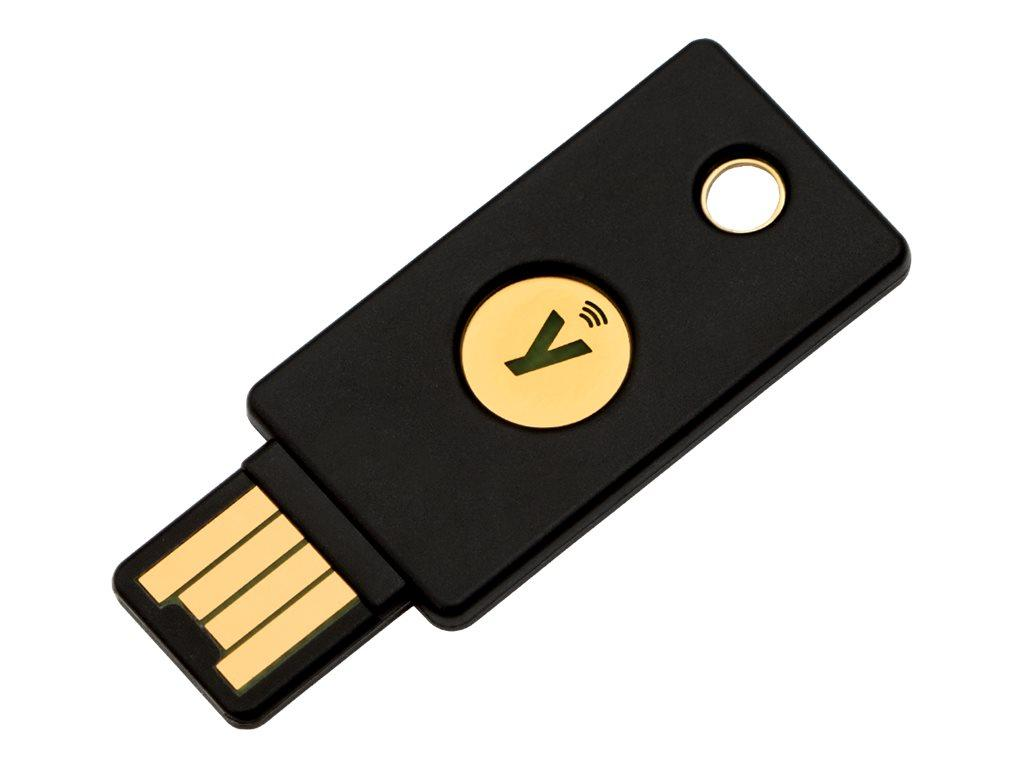
\includegraphics[width=0.3\textwidth]{img/abbildungen/yubikey.jpeg}
	\captionsetup{format=hang}
	\caption{Umsetzungsmöglichkeit mit Keycloak}
\end{figure}

 \begin{itemize}
    \item Ein Security Key ist eine Hardware, welche es ermöglicht einen Nutzer zu authentifizieren, indem dieser mit dem Security Key interagiert (beispielsweise durch einen Knopfdruck) \cite{reynolds2018tale}.
    \item Häufig werden Security Keys so designed, dass sie per USB an einen Computer angeschlossen werden können \cite{reynolds2018tale}.
    \item Die YubiKeys 5 ermöglichen drei Arten der Authentifizierung:
    1. \ac{SFA} Ersetzt Passwörter durch ein passwortloses \textit{tap-n-go} Verfahren.
    2. \ac{2FA} Sichert ein Passwort zusätzlich mit einem \textit{tap-n-go} Faktor ab. Der Security ist somit der zweite Faktor (\textit{something you have}).
    3. \ac{MFA} Verbindet die passwortlose \textit{tap-n-go} Authentifizierung mit einer PIN. (EIG AUCH SFA ODER NICHT)
 \end{itemize}

\subsection{Usability}

\begin{itemize}
    \item Vorteile:
    \item Ergebnisse zeigen, dass Nutzer grundsätzlich bereit sind, Passwörter durch passwortlose Verfahren zu ersetzen \cite{lyastani2020fido2}.
    \item Passwortlose Verfahren mit Yubikey wurden mehr akzeptiert als tradionelle passwortbasierte Verfahren \cite{lyastani2020fido2}.
    \item Implizite Garantie, dass sich lediglich Nutzer authentifizieren können, welche auch im Besitz des Authentifizierungsgerätes sind. \cite{lyastani2020fido2}.
    \item Durch die Nutzung von FIDO2 kann die Usability verbessert werden, da Nutzer sich keine Passwörter mehr merken müssen. Häufig wird das Verwalten der immer höher werdenden Anzahl an Passwörtern als Problem angesehen \cite{lyastani2020fido2} \cite{farke2020you}.
    \item Es wird ein deutlich geringerer kognitiver Aufwand benötigt, da Nutzer keine neuen Passwörter mehr erstellen und merken müssen \cite{lyastani2020fido2}.
    \item Zum aktuellen Zeitpunkt wird FIDO2 bereits von einer Vielzahl an Browsern unterstützt. Zusätzlich bieten immer mehr Online-Dienste die Möglichkeit an sich mit Hilfe von FIDO2 zu authentifizieren \cite{lyastani2020fido2} \cite{farke2020you}.
    \item Es handelt sich um offene und standardisierte Protokolle \cite{farke2020you}.
    \item Nachteile:
    \item Im Falle einer \ac{SFA} wird der Verlust des Authentifizierungsgerätes als größtes Problem angesehen. Bei Verlust hat auch der Nutzer keinen Zugriff mehr und aktuell gibt es noch keine sichere und effiziente Möglichkeiten, um den Zugriff wiederherzustellen (vor allem ohne Pause) \cite{lyastani2020fido2}.
    \item Da es sich um zusätzliche Hardware handelt kann diese ebenfalls kaputt gehen \cite{farke2020you}.
    \item Im Unternehmenskontext, kann die Verwaltung und Verteilung der Authentifizierungsgeräte zu einem Problem werden \cite{farke2020you}. 
    \item Da es sich um Hardware handelt, können Zugänge nicht an vertraute Personen weitergegeben werden, da der Zugang nur mit dem Authentifizierungsgerät möglich ist \cite{lyastani2020fido2}.
    \item Ohne das Authentifizierungsgerät sind keine spontanen Logins möglich \cite{lyastani2020fido2}.
    \item Es wird ein physischer Aufwand benötigt, da das Authentifizierungsgerät mitgeführt werden muss \cite{lyastani2020fido2}.
    \item Bereits das aus der Tasche holen des Authentifizierungsgerätes ist für manche Nutzer bereits eine Hürde \cite{farke2020you}.
    \item Authentifizierungsgeräte sind häufig mit Kosten verbunden, welche vom Nutzer getragen werden müssen \cite{lyastani2020fido2}.
    \item Nutzer haben Probleme ein neues Verfahren für die Authentifizierung zu nutzen, da sie sich an das alte Verfahren gewöhnt haben. Das führt dazu, dass Nutzer das neue Verfahren als kompliziert und ungewohnt empfinden. Sie verfügen häufig nicht über das nötige Wissen, um die Funktion und Sicherheit des Verafahrens zu verstehen \cite{lyastani2020fido2}.
    \item Selbst Nutzern, welchen das Konzept der passwortlosen Authentifizierung gefällt, nutzen häufig weiterhin Passwörter \cite{farke2020you}.
    \item Nutzer wollen keine Angewohnheiten verändern, wenn die nicht dazu gezwungen sind \cite{farke2020you}.
    \item Nutzer verwenden lieber Passwörter, da sie das Konzept und die Technologie besser verstehen \cite{lyastani2020fido2}.
    \item Nicht zwangsweise schneller als die Nutzung von Passwortmanagern \cite{farke2020you}.
    \item Allgemein fällt das Feeback von Nutzern weniger positiv aus, wenn diese vorher bereits Passwortmanager genutzt haben \cite{farke2020you}.
    \item Fazit:
    \item Insgesamt lassen sich noch nicht alle Szenarien mit FIDO2 abdecken. Es gibt noch spezielle Fälle, in welchen die Nutzung von Passwörtern weiterhin notwendig ist \cite{lyastani2020fido2}.
    \item 
\end{itemize}

\section{Fido2} \label{fido2}

\begin{figure}[h]
	\centering 
	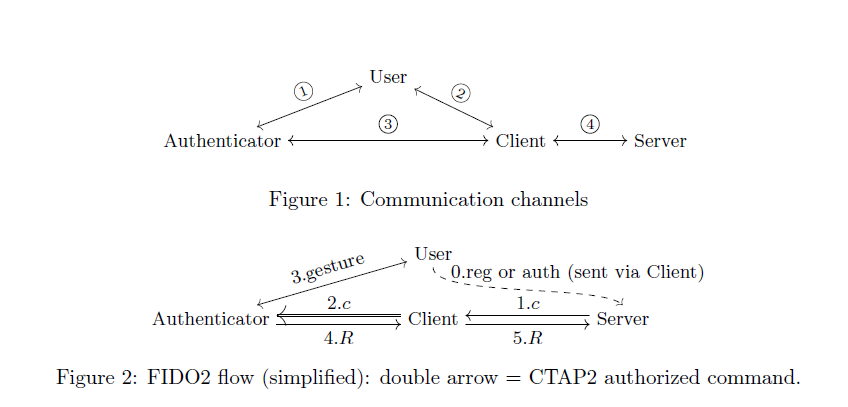
\includegraphics[width=1\textwidth]{img/abbildungen/fido2-simple.png}
	\captionsetup{format=hang}
	\caption{Umsetzungsmöglichkeit mit Keycloak}
\end{figure}

\begin{figure}[h]
	\centering 
	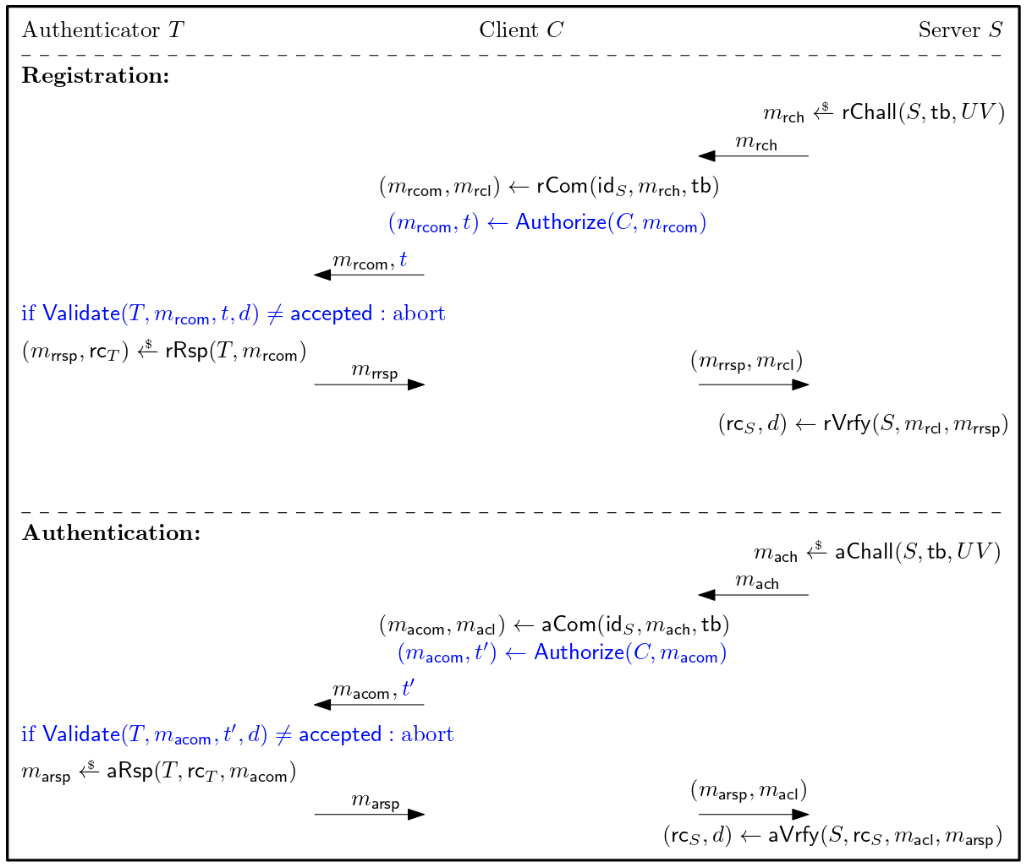
\includegraphics[width=1\textwidth]{img/abbildungen/Fido2.png}
	\captionsetup{format=hang}
	\caption{Umsetzungsmöglichkeit mit Keycloak}
\end{figure}

\begin{figure}[h]
	\centering 
	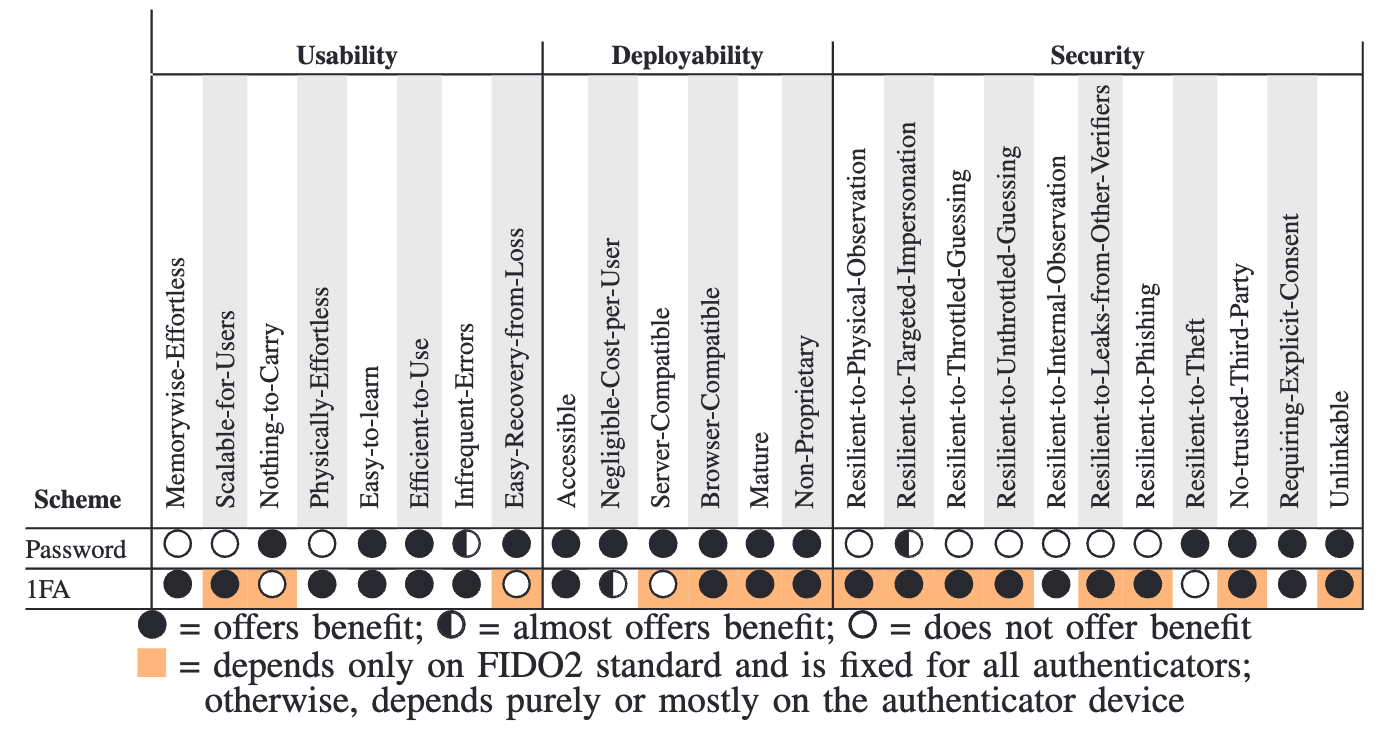
\includegraphics[width=1\textwidth]{img/abbildungen/fido2_usability.png}
	\captionsetup{format=hang}
	\caption{Umsetzungsmöglichkeit mit Keycloak}
\end{figure}

\begin{itemize}
    \item FIDO2 wird von der \ac{FIDO} und dem \ac{W3C} entwickelt und bereitgestellt \cite{lyastani2020fido2} \cite{farke2020you}.
    \item Die \ac{FIDO} Allianz ist eine Organisation mit weltweit über 250 Mitgliedern. Darunter befinden sich Unternehmen wie Google, Microsoft, Apple Amazon, Facebook, Visa und viele mehr \cite{lyastani2020fido2} \cite{farke2020you}.
    \item Ziel ist es Nutzer zu authentifizieren, ohne, dass diese eine Passwort nutzen müssen \cite{morii2017research} \cite{barbosa2021provable}.
    \item Basiert auf der Nutzung eines internen oder externen Authentifizierungsgerätes \cite{morii2017research} \cite{barbosa2021provable}.
    \item Dabei können Authentifizierungsgeräte, ebenfalls mit einer PIN oder einem biometrischen Merkmal, geschützt werden \cite{farke2020you}.
    \item Hierbei ist ein PIN allerdings nicht gleichzusetzen mit einem Passwort. Der PIN wird lediglich für das Authentifizierungsgerät genutzt und wird auch nur auf diesem gespeichert \cite{farke2020you} \cite{barbosa2021provable}.
    \item Es handelt sich dabei also auch nicht um eine \ac{MFA}, sondern, um einen einzelnen Faktor, welcher lediglich den Zugriff das Gerät selbst authentifiziert \cite{barbosa2021provable}.
    \item FIDO2 unterstützt sowohl \ac{MFA} als auch \ac{SFA} \cite{lyastani2020fido2} \cite{farke2020you}.
    \item Viele Alternativen zur passwortbasierten AUthentifizierung existieren bereits. Diese werden allerdings nur in einem sehr geringen Ausmaß genutzt \cite{farke2020you}.
    \item Stellt Zugangsdaten bereit, welche nicht gephisht oder von Datenlecks betroffen sein können \cite{lyastani2020fido2}.
    \item Das liegt daran, dass keine geteilten Geheimnisse zwischen Nutzer und Dienst existieren, welche auf einem Server gespeichert werden \cite{morii2017research}.
    \item Wird von fast allen Browsern standardmäßig unterstützt \cite{lyastani2020fido2}.
    \item Viele verfügbare Authentifizierungsgeräte. Z.B. Security Keys oder auch Smartphones. Beispielsweise Apples Touch ID oder Face ID \cite{lyastani2020fido2}.
    \item Besteht aus zwei Komponenten: CTAP2 für die Kommunikation zwischen Client und Authentifizierungsgerät und WebAuthn für die Kommunikation zwischen Client und Server \cite{farke2020you}.
    \item Dabei wird WebAuthn von der \ac{W3C} spezifiziert und CTAP2 von der \ac{FIDO} Allianz \cite{farke2020you}.
\end{itemize}

\subsection{Webauthn}

\begin{itemize}
    \item WebAuthn ist ein Standard, welcher von dem \ac{W3C} entwickelt wird. Das Protokoll erlaubt es Webanwendungen Nutzer zu authentifizieren. Dies kann dabei auch über \ac{CTAP2} erfolgen \cite{lyastani2020fido2}. ?
    \item Wurde 2019 ein offizieller Webstandard \cite{farke2020you}.
    \item Spezifiziert eine standardiserte, vom Browser unabhängige JavaScript API zur Authentifizierung von Nutzern für Webanwendungen. So können Webanwendungen eine Authentifizierung integrieren, welche resistent gegenüber Phishing, Datenlecks und Passwortdiebstahl ist. Anstelle von geteilten Geheimnissen nutzt WebAuthn public-key Kryptographie, um einzigartige Zugangsdaten für jede Webanwendung zu erstellen, welche nur auf dem Gerät des Nutzers gespeichert werden \cite{farke2020you}.
    \item Passwortloses Challenge-Response-Verfahren zwischen Client und Server \cite{barbosa2021provable}.
    \item WebAuthn unterstützt zwei Opertationen: Registrierung und Anmeldung \cite{barbosa2021provable}.
    \item In der Registrierungsphase sendet der Server dem Authentifizierungsgerät über den CLient eine zufällige Challenge. In dieser Phase signiert das Authentifizierungsgerät mit Hilfe seines privaten Schlüssels die CHallenge und sendet zusätzlich  öffentliche Anmeldedaten für zukünftige Anmeldungen an den Server. Meldet sich ein bereits registrierter Nutzer an, wird die Challenge des Servers erneut von dem Authentifizierungsgerät signiert zurück an den Server gesendet. Der Server kann die Signatur mit Hilfe des öffentlichen Schlüssels verifizieren und den Nutzer authentifizieren \cite{barbosa2021provable}.
    \item Registrierungsphase:
    Der Server \textit{S} sendet eine challenge message $m_{rch}$ über den Client \textit{C} an den Security Key. Diese Challenge beinhaltet eine randomisierte Nonce, Parameter (beispielsweise, ob eine Nutzerverifizierung notwendig ist) und optional einen wert \textit{tb}, welcher den zugrunde liegenden Kanal eindeutig identifiziert (typischerweise eine \ac{TLS} Verbindung). Der Client \textit{C} erhält die challenge message $m_{rch}$ und wandelt diese in eine command message $m_{rcom}$ und eine client mesasage $m_{rcl}$ um. die command message $m_{rcom}$ wird an den Security Key $T$ übermittelt. Der Security Key $T$ erzeugt öffentlich-privates Schlüsselpaar, welches an den Server $S$ gebunden ist und diesem ermöglicht eine Verifizierung, während der folgenden AUthentifizierungsphase durchzuführen. Zudem gibt der Security Key $T$ eine response message $m_{rrsp}$ aus. Der Client übergibt diese und die client message $m_{rcl}$ an den Server $S$. Die response message $m_{rrsp}$ beinhaltet einen \textit{attestation type}, welcher es dem Server $S$ ermöglicht eine Verifizierung während der Registrierungsphase durchzuführen und beinhaltet den öffentlichen Schlüssel. WebAuthN 2 unterstützt fünf \textit{attestation types}. Häufig werden die types \textit{None} und \textit{Basic} verwendet. Die restlichen types sind \textit{Self}, \textit{AttCA} und \textit{AnonCA}. \cite{bindel2022fido2}
    \item Authentifizierungsphase:
    Der Client empfängt die challenge message $m_{ach}$ von Server $S$ und wandelt diese in eine command message $m_{acom}$ und eine client message $m_{acl}$ um. Die command message $m_{acom}$ wird an den Security Key $T$ übermittelt. Der Security Key $T$ erzeugt eine response message $m_{arsp}$, welche mit dem privaten Schlüssel signiert wird und sendet diese an den Server $S$ (über den Client $C$). Der Server $S$ akzeptiert die response message $m_{arsp}$ und die client message $m_{acl}$ nur, wenn sie sich mit dem dazugehörigen öffentlichen Schlüssel verifizieren lassen. \cite{bindel2022fido2}
    \item Die Sicherheit von WebAuthn basiert auf dem Beweis, dass RSASSA PKCS1-v1\_5 und RSASSA-PSS als \ac{EUF-CMA} gelten und der Annahme, dass SHA-256 kollisionsresistent ist \cite{barbosa2021provable}.
\end{itemize}

\subsection{CTAP2}
\begin{itemize}
    \item 2018 wurde \ac{CTAP2} als internationaler Standard der \ac{ITU-T} anerkannt \cite{barbosa2021provable}.
    \item \ac{CTAP2} ist ein Protokoll auf der Anwendungsebene, welches für die Kommunikation zwischen eines WebAuthn Clients und eines konformen Authentifizierungsgerätes genutzt wird. Das Authentifizierungsgerät kann dabei ein externes Gerät sein wie beispielsweise ein Security Key, welches über USB, Bluetooth oder NFC eine Verbindung mit dem Client aufbaut. Aber auch ein internes Gerät wie beispielsweise ein Fingerabdruckscanner oder ein Trusted Platform Module können als Authentifizierungsgerät genutzt werden \cite{lyastani2020fido2}.
    \item \ac{CTAP2} spezifiziert, die Kommunikation zwischen einem Authentifizierungsgerät und einem Client. Der Client ist dabei üblicherweise ein Webbrowser. Das Ziel ist es zu garantieren, dass der CLient das AUthentifizierungsgerät nur nutzen darf, wenn der Nutzer dies erlaubt. Dafür muss der Nutzer beispielsweise einen Knopf am Authentifizierungsgerät drücken und/oder sich mit Hilfe eines PINs oder eines biometrischen Merkmals beim AUthentifizierungsgerät authentifizieren \cite{barbosa2021provable}.
    \item Das Ziel ist es somit einen Client an das AUthentifizierungsgerät zu binden. Ist ein CLient nicht an das authentifizerungsgerät gebunden, kann dieser sich nicht authentifizieren \cite{barbosa2021provable}.
    \item besteht aus mehreren Phasen. 
    1. In der Setup Phase initialisiert ein Client $C'$ einen PIN, welcher vom User übergeben wird an den Security Key $T$.
    2. In der Binding Phase tauschen ein Client $C$ (nicht zwangsweise $C'$) und der Security Key $T$ einen gemeinsamen Verbindungsstatus aus, wenn der Client $C$ in der Lage ist, Informationen über die auf dem Security Key $T$ gespeicherte PIN zu liefern. So soll eine einzigartige Verbindung zwischen dem Client $C$ und dem Security Key $T$ hergestellt werden. Schlägt der Client $C$ drei mal in Folge fehl die PIN zu liefern, wird der Security Key $T$ neu gestartet und der Verbindungsstatus wird zurückgesetzt. Schlägt der Client $C$ insgesamt acht mal fehl, wird der Security Key $T$ gesperrt.
    3. Ist diese Phase erfolgreich, autorisiert der Client $C$ jeden Befehl, indem eer einen Tag $t$ ausgibt, welcher mit der command message an den Security Key $T$ übermittelt wird. Der Security Key $T$ fährt lediglich fort, wenn eine \textit{positive decision} $d$ des Users vorliegt (beispielsweise einem Knopfdruck) und validiert darauf hin die command message und den Tag $t$. \cite{bindel2022fido2}
    \item \ac{CTAP2} nutzt unauthentifizierten Diffie-Hellman Schlüsselaustausch \cite{barbosa2021provable}.
    \item Dieser kann von \ac{MITM} Angriffen betroffen sein \cite{barbosa2021provable}.
    \item In der Binding Phase sendet das Authentifizierungsgerät dem CLient ein pinToken, welcher beim hochfahren des Authentifizierungsgerätes generiert wird. Dieser pinToken wird lokal auf dem AUthentifizierungsgerät gespeichert und wird von dem verbundenen Client in der Access Channel Phase genutzt, um die nachfolgenden Nachrichten des Clients zu autorisieren \cite{barbosa2021provable}.
    \item Jedem AUthentifizierungsgerät wird ein pinToken pro hochfahren zugeordnet. Das bedeutet mehrere CLients erezugen mehrere Access Channels mit dem selbem Authentifizierungsgerät und dem selben pinToken \cite{barbosa2021provable}.
    \item Dadurch wird die Sicherheit von \ac{CTAP2} limitiert ??
\end{itemize}

\subsubsection{CTAP2.1}
\begin{itemize}
    \item Gilt in Verbindung mit WebAuthn 2 als \ac{PQ} bereit, da ein Operationsmodus ermöglicht wird, der nur kryptographische Primitive, digitale Signaturen und \ac{KEM} verwendet \cite{bindel2022fido2}.
    \item Im Gegensatz zu \ac{CTAP2} basiert CTAP2.1 nicht auf unauthentifizierten Diffie-Hellman Schlüsselaustausch, sondern auf einem sogeannten \ac{puvProtocol}, wodurch die \ac{PQ}-Sicherheit ermöglicht wird \cite{bindel2022fido2}.
    \item In \ac{CTAP2} wird der Verbindungszustand als \textit{pinToken} definiert, welcher aus mehreren 128 Bit-Blöcken besteht und keine maximale Begrenzung der Länge beseitzt. In CTAP2.1 wird der Verbindungszustand als \textit{pinUvAuthToken} definiert welcher eine feste Länge von 128 oder 256 Bit besitzt \cite{bindel2022fido2}.
    \item Der pinToken von \ac{CTAP2} wird bis zum nächsten Neustart wiederverwendet. Der pinUvAuthToken von CTAP2.1 wird nach jeder erfolgreichen Authentifizierung neu generiert. Das führt dazu, dass CTAP2.1 eine \ac{SUF}-t' Sicherheit aufweist und \ac{CTAP2} lediglich eine \ac{UF}-t' Sicherheit \cite{bindel2022fido2}.
    \item \ac{CTAP2} erlaubt es Security Keys und Clients nur den pinUvAuthToken zu teilen, wenn der Nutzer den korrekten PIN eingegeben hat. CTAP2.1 ermöglicht zusätzlich, dass der Nutzer sich mit Hilfe eines biometrischen Merkmals authentifiziert \cite{bindel2022fido2}.
\end{itemize}

\subsection{Sicherheit}

\begin{itemize}
    \item FIDO2 ist eine Erweiterung des FIDO U2F Protokolls und bietet die selbe Sicherheit wie public key Kryptographie \cite{lyastani2020fido2}.
    \item Es handelt sich um geprüfte assymetrische Kryptographie \cite{farke2020you}.
    \item Es handelt sich dabei um ein Challenge-Response-Verfahren mittels Hardware basierten Authentifizierungsgeräten. Dies bietet einige Vorteile gegenüber passwortbasierten Verfahren. Es gibt keine geteilten Geheimnisse zwischen Usern und Diensten, welche durch Phishing oder Datenlecks kompromittiert werden können. Dabei ist das selbe Authentifizierungsgerät für mehrere Dienste nutzbar, ohne, dass sich dabei eine Verknüpfung zurückführen lässt \cite{lyastani2020fido2} \cite{farke2020you}.
    \item lediglich die Session kann kompromittiert werden \cite{morii2017research}.
    \item Authentifizierungsgeräte lassen sich mit zusätzlichen PINs oder biometrischen Merkmalen absichern, um sich ebenfalls vor Diebstahl schützen \cite{barbosa2021provable}.
    \item Unauthentifizierter Diffie-Hellman Schlüsselaustausch könnte durch ein \ac{PAKE} Verfahren ersetzt werden \cite{barbosa2021provable}.
    \item Das Paper gibt an, dass dieses sicherer und effizienter sein soll \cite{barbosa2021provable}.
    \item In folgendem Szenario: 1. Der Nutzer besitzt einen Security Key, welcher mit einem drückbaren Knopf oder ähnlichen ausgestattet ist. 2. Der Security Key ist mit einem geheimen PIN geschützt. 3. Der Nutzer autorisiert vertrauten Clients auf den Security Key zuzugreifen. 4. Der Nutzer verbindet seinen Security Key mit mehreren Clients und nutzt diese um sich bei mehreren Webdiensten zu registrieren/anzumelden.
    Dann ist versichert, dass:
    1. Die Authentifizierung von dem Security Key durchgeführt wurde, welcher die genutzen Zugangsdaten bei dem Webdienst registriert hat.
    2. ein autorisierter Befehl auf den Security Key zugegriffen hat.
    3. und dieser autorisierte Befehl von einem autorisierten Client beauftragt wurde (sollte der Nutzer den korrekten PIN eingegeben haben).
    Dies setzt voraus, dass:
    1. Der Security Key nicht gestohlen wurde.
    2. Der PIN des Security Keys nicht kompromittiert wurde.
    3. Der autorisierte Client nicht kompromittiert wurde (korrekte Ausführung von \ac{CTAP2} und CLient ist nicht von böswilliger Software betroffen).
    \cite{barbosa2021provable}.
    \item Wird ein Security Key gestohlen, kann dieser nur genutzt werden, wenn ebenfalls der PIN bekannt ist \cite{barbosa2021provable}.
\end{itemize}


\chapter{Umsetzung}

Im Folgenden wird die Umsetzung einer Integration eines Security Keys in Kombination mit \ac{FIDO}2 innerhalb der \ac{LSY} beschrieben. Dabei wird der aktuelle Stand berücksichtigt und begründet ein passender Ansatz für die Integration gewählt. Zusätzlich wird die Umsetzung zum Aspekt der Benutzerfreundlichkeit analysiert.

\section{Aktueller Stand der LSY}
Innerhalb der \ac{LSY} werden aktuell verschiedene Verfahren zur Authentifizierung genutzt. Grundsätzlich besteht eine zentrale Nutzerverwaltung innerhalb der \ac{LSY}, welche innerhalb einer Microsoft Azure \ac{AD} verwaltet wird. Wie diese an eine Applikation gebunden ist, ist dabei nicht vorgegeben und kann von den jeweiligen ABteilungen individuell festgelegt werden. Auch Lösungsansätze ohne die Nutzung der Azure \ac{AD} sind je nach Abteilung möglich. Die einzige zentrale Schnittstelle ist somit die genannte Azure \ac{AD}.

Diese bestehende Nutzerverwaltung basiert auf einer passwortbasierten Authentifizierung inklusive \ac{MFA}. Das Passwort muss von allen Nutzern in regelmäßigen Abständen (drei Monate) geändert werden. Der weitere Faktor für die Nutzung der \ac{MFA} kann frei von den Nutzern gewählt werden, solange er mit der Azure \ac{AD} kompatibel ist. Zusätzlich zur regelmäßigen Passwortänderungen, gibt es Richtlinien zur Passworterstellung, welche von den Nutzern eingehalten werden müssen. 

Grundsätzlich ist eine Integration eines Security Keys als \ac{SFA} mit Hilfe einer Azure \ac{AD} möglich. Auch als zweiten Faktor für eine \ac{MFA} kann ein Security Key genutzt werden. Diese Funktion ist innerhalb der \ac{LSY} allerdings nicht aktiviert, da diese Art der Authentifizierung nicht den Richtlinien des Unternehmens entspricht. Eine Änderung dieser Richtlinien ist möglich, erfordert allerdings einen sehr hohen Aufwand und viel Zeit. Da der Bearbeitungsraum dieser Arbeit zeitlich limitiert ist, wird aus den genannten Gründen keine \ac{LSY} weite Integration eines Security Keys betrachtet. Dennoch soll eine Integration in einem kleinerem Rahmen auf Abteilungsebene getestet werden. Dies soll eine Aussage ermöglichen, ob eine Umstellung der aktuellen Richtlinien sinnvoll ist und eine Integration eines Security Keys in der gesamten \ac{LSY} möglich ist.

Für diese Testphase wird die Abteilung cGroup Solutions ausgewählt. Diese ist zuständig für das Produkt cFront, welches in \textbf{\ref{cFront-exp}} beschrieben ist. Innerhalb der Abteilung wird aktuell eine passwortbasierte Authentifizierung gegen die Azure \ac{AD} inklusive \ac{MFA} genutzt. Vorteilhaft für die Integration eines Security Keys ist, dass die Abteilung zusätzlich Keycloak für die Identitäts- und Zugriffsverwaltung nutzt. Keycloak ist eine Open-Source-Plattform für Identitäts- und Zugriffsmanagement, die Single Sign-On, Benutzerverwaltung und Sicherheitsfunktionen bietet, um die Authentifizierung und Autorisierung in Anwendungen zu erleichtern. Es wird verwendet, um Benutzer sicher anzumelden, ihre Zugriffsrechte zu verwalten und die Integration mit anderen Identitätsdiensten zu unterstützen \cite{keycloak}. Somit bietet sich eine neue Schnittstelle für die testweise Integration eines Security Keys an, da Keycloak zwar die Schnittstelle zur Azure \ac{AD} nutzt, allerdings zusätzlich auch eine eigene Nutzerverwaltung besitzt. Dies erfordert keine Änderungen der aktuellen Richtlinien oder große technische Umstellungen innerhalb der gesamten \ac{LSY}, sondern ermöglicht eine Integration auf Abteilungsebene.

Die aktuelle Umsetzung der Abteilung zur Authentifizierung ist vereinfacht in \textbf{\ref{current-imp}} abgebildet. Die Applikation kommuniziert nicht direkt mit dem Keycloak-Server, sondern nutzt eine selbst entwickelte Anwendung, welche sich als Keycloak-Client ausgibt. Der Nutzer gibt seine Zugangsdaten bei der Anmeldung an den Keykloak-Client weiter. Dieser wandelt die Zugangsdaten in einen validen JWT-Token um und übergibt diesen an den Keycloak-Server. Der Keycloak-Server validiert die Zugangsdaten gegen die Azure \ac{AD} und authentifiziert den Nutzer, indem er einen oAuth2-Token erstellt und diesen an die Applikation zurückgibt.


\begin{figure}[h]
	\centering 
	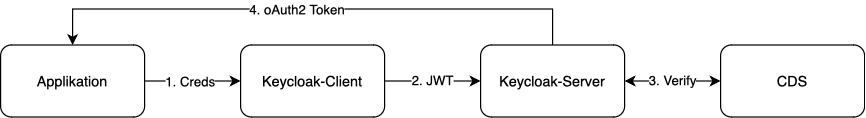
\includegraphics[width=1\textwidth]{img/abbildungen/Unknown.png}
	\captionsetup{format=hang}
	\caption{Aktuelle Umsetzung der Abteilung} \label{current-imp}
\end{figure}

\section{Wahl des Security Keys} \label{secwahl}
Für die Umsetzung der passwortlosen Authentifizierung innerhalb der \ac{LSY} wurde ein Yubikey der Series 5 mit NFC gewählt. Dieser wurde in Kapitel vorgestellt. Hingewiesen sei an dieser Stelle, dass auch andere Hersteller Security Keys anbieten, welche das FIDO2-Protokoll unterstützen. 

Dazu gehören unter anderem:
\begin{itemize}
    \item \textit{Feitian ePass} des Herstellers FEITIAN Technologies Co., Ltd.
    \item \textit{Titan} des Herstellers Google
    \item \textit{SafeNet eToken} des Herstellers Thales Group
\end{itemize}

Die Wahl des Security Keys richtete sich allerdings unter anderem an der Kompatibilitätsliste \cite{compWin} von Microsoft. Diese listet alle Security Keys auf, welche für eine passwortlose Authentifizierung gegen eine Microsoft Azure \ac{AD} genutzt werden können. Nicht auffindbar in der Liste ist beispielsweise der Google Titan. Dieser unterstützt aktuell nicht FIDO2, sondern lediglich FIDO und \ac{U2F}. Microsoft ist allerdings nicht abwärtskompatibel, was bedeutet, dass der Google Titan nicht für eine passwortlose Authentifizierung gegen das Azure \ac{AD} genutzt werden kann \cite{seckeytest}.

Die endgültige Auswahl basiert auf dem bestehenden Bestand eines Yubikeys der Series 5 mit NFC. Dieser ist mit der Azure \ac{AD} nutzbar. Grundsätzlich ist allerdings auch eine Nutzung eines anderen Security Keys möglich, sofern dieser das \ac{FIDO}2-Protokoll unterstützt, in der Kompatibilitätsliste von Microsoft aufgeführt ist und und offiziel von der \ac{FIDO} Allianz zertifiziert wurde.

Sollte die Nutzung eines Security Keys innerhalb der \ac{LSY} in Zukunft erweitert werden, so wird eine neue weitreichende Analsyse notwendig. Da im Rahmen dieser Arbeit lediglich eine Testphase auf Abteilungsebene stattfindet und die grundsätzliche Funktionsweise der unterschiedlichen Security Keys ähnlich ist, wird auf eine detaillierte Analyse der unterschiedlichen Security Keys verzichtet.

\section{Integration eines Yubikeys in die LSY}

\begin{figure}[h]
	\centering 
	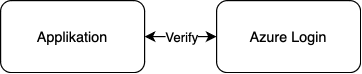
\includegraphics[width=0.6\textwidth]{img/abbildungen/azure_umsetzung.png}
	\captionsetup{format=hang}
	\caption{Umsetzungsmöglichkeit mit Azure \ac{AD}}
\end{figure}

\begin{itemize}
    \item Grundsätzlich gibt es zwei Möglichkeiten in die aktuelle Applikation eine passwortlose Authentifizierung mit Hilfe eines Yubikeys zu integrieren: Die Nutzung der Authentifizierung gegen das Azure \ac{AD} oder die eine veränderte Nutzung der aktuellen Keycloak-Lösung.

\end{itemize}

Eine Lufthansa-weite Policy für die Nutzung der Azure \ac{AD} verbietet allerdings die Nutzung eines Security Keys für eine \ac{SFA}. Hier kann der Security Key lediglich als zweiter Faktor genutzt werden. Dies kann jeder Nutzer selber verwalten. Registriert ein Nutzer seinen Security Key in seinem Profil, erscheint bei der Anmeldung (nach der Eingabe des Passwortes) ein zusätzliches Feld:

\begin{figure}[h]
	\centering 
	
\includegraphics[width=0.6\textwidth]{img/abbildungen/azure_seckey.png}
	\captionsetup{format=hang}
	\caption{Umsetzungsmöglichkeit mit Keycloak}
\end{figure}

Verwendet der Nutzer einen Security Key wird dieser im Folenden aufgefordert die zugehörige PIN einzugeben und den Knopf des Security Keys zu drücken. Grundsätzlich ist eine passwortlose Authentifizierung mit Hilfe eines Security Keys innerhalb der Azure \ac{AD} möglich. Da eine Änderung dieser Lufthansa Policy notwendig wäre, übersteigt dies allerdings den Rahmen dieser Arbeit.

Da allerdings aktuell eine beschriebene Nutzung von Keycloak stattfindet und Keycloak eine passwortlose Authentifizierung mit Hilfe eines Security Keys unterstützt, wäre eine Umsetzung mit Hilfe von Keycloak möglich. Hierbei wird die aktuelle Lösung verändert und entsprechend angepasst:

\begin{figure}[h]
	\centering 
	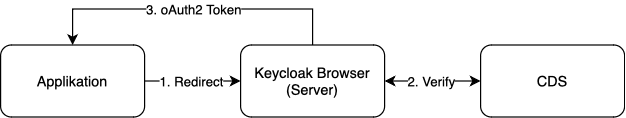
\includegraphics[width=1\textwidth]{img/abbildungen/keycloak_browser.png}
	\captionsetup{format=hang}
	\caption{Veränderter Keycloak-Login}
\end{figure}

Statt bei einer Anmeldung einen Client zu simulieren bietet Keycloak die Möglichkeit eine Anmeldung über eine Nutzeroberfläche zu realisieren. Dafür wird ein redirect auf die Keycloak-Login-Seite durchgeführt. Bei einer erfolgreichen Verifizierung wird der Nutzer zurück auf die Applikation geleitet und vom Keycloak-Server mit Hilfe eines oAuth2-Tokens authentifiziert. 

Um eine Passwortlose Authentifizierung in Keycloak zu ermöglichen, muss der Authentication Flow für eine Browser-Anmeldung modifiziert werden. Der angepasste Authentication Flow besteht aus folgenden Schritten:

\begin{figure}[h]
	\centering 
	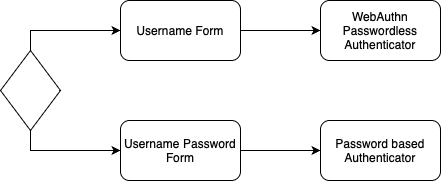
\includegraphics[width=0.7\textwidth]{img/abbildungen/authentication_flow.png}
	\captionsetup{format=hang}
	\caption{Authentication Flow}
\end{figure}

Hierbei wird die untere Hälfte der Grafik weiterhin ermöglicht, da es sich lediglich um einen Test handelt. Grundsätzlich wird diese nicht ermöglicht, da Keycloak eine reine passwortlose \ac{SFA} unterstützt.

Die obere Hälfte der Grafik entspricht dem für diese Arbeit relevanten Authentication Flow. Dabei wird der User zunächst aufgefordert seinen Nutzernamen einzugeben und anschließend seinen Security Key zu verwenden. Dies ist notwendig, um die Nutzung eines Security Keys für mehrere Zugänge zu ermöglichen. Ermöglicht man lediglich die Nutzung eines Zugangs pro Security Key, so wird die Eingabe des Nutzernamens nicht benötigt. Zusätzlich erfolgt eine Konfiguration des Keycloak-Servers, welche die Registrierung eines Security Keys bei der Registrierung eines neuen Nutzers ermöglicht.

Mit Hilfe dieser Konfiguration werden zwei Abläufe ermöglicht. Eine neue Registrierung:

\begin{figure}[H]
	\centering 
	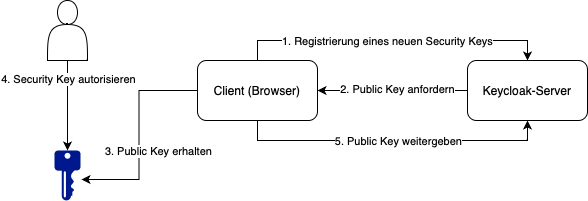
\includegraphics[width=1\textwidth]{img/abbildungen/register_simplified.png}
	\captionsetup{format=hang}
	\caption{Registrierung (vereinfacht)}
\end{figure}

Sowie eine neue Anmeldung:

\begin{figure}[H]
	\centering 
	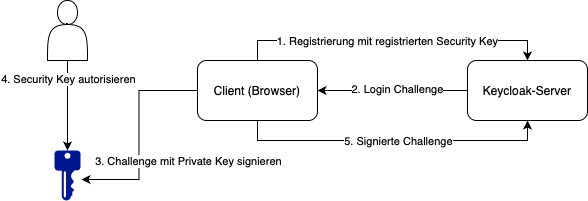
\includegraphics[width=1\textwidth]{img/abbildungen/login_simplified.png}
	\captionsetup{format=hang}
	\caption{Anmeldung (vereinfacht)}
\end{figure}

Die Grafiken stellen den vereinfachten Ablauf der Registrierung und Anmeldung mit Hilfe eines Security Keys dar. Die detailierte Darstellung der Funktionsweise ist in Kapitel 2.7 zu finden. Der entscheidende Unterschied der beiden Prozesse ist allerdings, dass bei der Registrierung lediglich der öffentliche Schlüssel übergeben wird, während bei der Anmeldung der private Schlüssel benötigt wird. Dieser wird allerdings nicht übergeben, sondern signiert eine Login Challenge, welche vom Keycloak-Server generiert wird. Kann der Keycloak-Server die Signatur mit Hilfe des gespeicherten öffentlichen Schlüssels verifizieren, wird der Nutzer authentifiziert. Sowohl die Registrierung als auch die Anmeldung erfolgen hierbei also nicht über die Anwendung selbst, sondern über den Keycloak-Server und dessen Nutzeroberfläche.

\section{User Feedback}
Um eine Aussage über die Akzeptanz und die Benutzerfreundlichkeit der aufgezeigten Umsetzung zu treffen, wird ein Feedback von den Nutzern der Abteilung cGroup Solutions eingeholt. Um eine wissenschaftliche Aussage zu treffen wird ein Fragebogen erstellt. Es handelt sich dabei um eine Mischform aus einer qualitativen und einer quantitativen Befragung. So wird es ermöglicht eine numerische Auswertung der Antworten zu erhalten, sowie eine qualitative Auswertung der Kommentare. Im Folgenden wird die Durchführung des Fragebogens beschrieben.

\subsection{Rahmen des Feedbacks}
Da zum Zeitpunkt der Erstellung dieser Arbeit die Nutzung keine Umsetzung einer passwortlosen Authentifizierung innerhalb der gesamten \ac{LSY} möglich ist (siehe Kapitel) wird das Feedback auf die Abteilung cGroup Solutions beschränkt. Diese ist zuständig für das in Kapitel beschriebene Produkt cFront, in welchem die passwortlose Authentifizierung testweise implementiert wurde. Die Abteilung besteht aus 15 Personen.

Über einem Zeitraum von zwei Wochen werden alle Mitglieder eingeladen an der Befragung teilzunehmen. Eine Teilnahme ist freiwillig. Die Befragung findet im Büro der Abteilung statt und wird von dem Autor dieser Arbeit durchgeführt. Jeder Teilnehmer wird einzeln und vor Ort befragt. Dies ermöglicht es mit jedem Teilnehmer eine Live-Demonstration durchzuführen. So wird ebenfalls ermöglicht, dass Teilnehmer bereits während der Befragung und der Demonstration Kommentare hinterlassen können. Diese werden auf dem Fragebogen festgehalten und werden für die qualitative Auswertung genutzt werden.

Während der gesamten Demonstration und Befragung werden den Teilnehmern keine Informationen zum Fido2 Protkoll vermittelt, da sonst die Aussagekraft des Feedbacks verfälscht werden könnte. Ziel ist es den ersten Eindruck aller Teilnehmer zu erhalten, ohne dass diese eine erzwungene Einführung in die Thematik erhalten. Die Live-Demonstration beinhaltet die Registrierung und Anmeldung mit Hilfe eines Security Keys, sowie eine Demonstration einer möglichen Anmeldung mit Hilfe eines Passkeys. Zusätzlich erhalten die Teilnehmer die Möglichkeit den Security Key physich zu betrachten. Ein detailierter Verlauf der Demonstartion wird im weiteren Verlauf der Arbeit beschrieben.

\subsection{Auswahl der Teilnehmer}
Zur Durchführung des Fragebogens wurden alle Mitglieder des Teams eingeladen, eine Teilnahme war jedoch freiwillig. Zwei der Mitglieder der Abteilung konnten auf Grund eines Urlaubs nicht an der Befragung teilnehmen. Vor der Durchführung wurden alle Teilnehmer darüber informiert zu welchem Zweck die Daten für diese Arbeit erhoben werden. Die Befragung stand dabei nicht anonym statt, um einen Austausch zwischen dem Autor und den Teilnehmern zu ermöglichen. Da die Befragung die Abteilung der Teilnehmer betrifft sollten diese somit eine Möglichkeit bekommen, ihre Gedanken zu dem modifiziertem Anmeldevorgang zu teilen.

14 Mitglieder der Abteilung stimmten der Teilnahme an der Befragung zu. Die letzte Person befand sich während des möglichen Zeitraumes der Befragung im Urlaub. Das durchschnittsalter der Teilnehmer beträgt 45,4 Jahre. Die genaue Verteilung wird in der folgenden Grafik sichtbar:

\begin{figure}[h]
	\centering 
	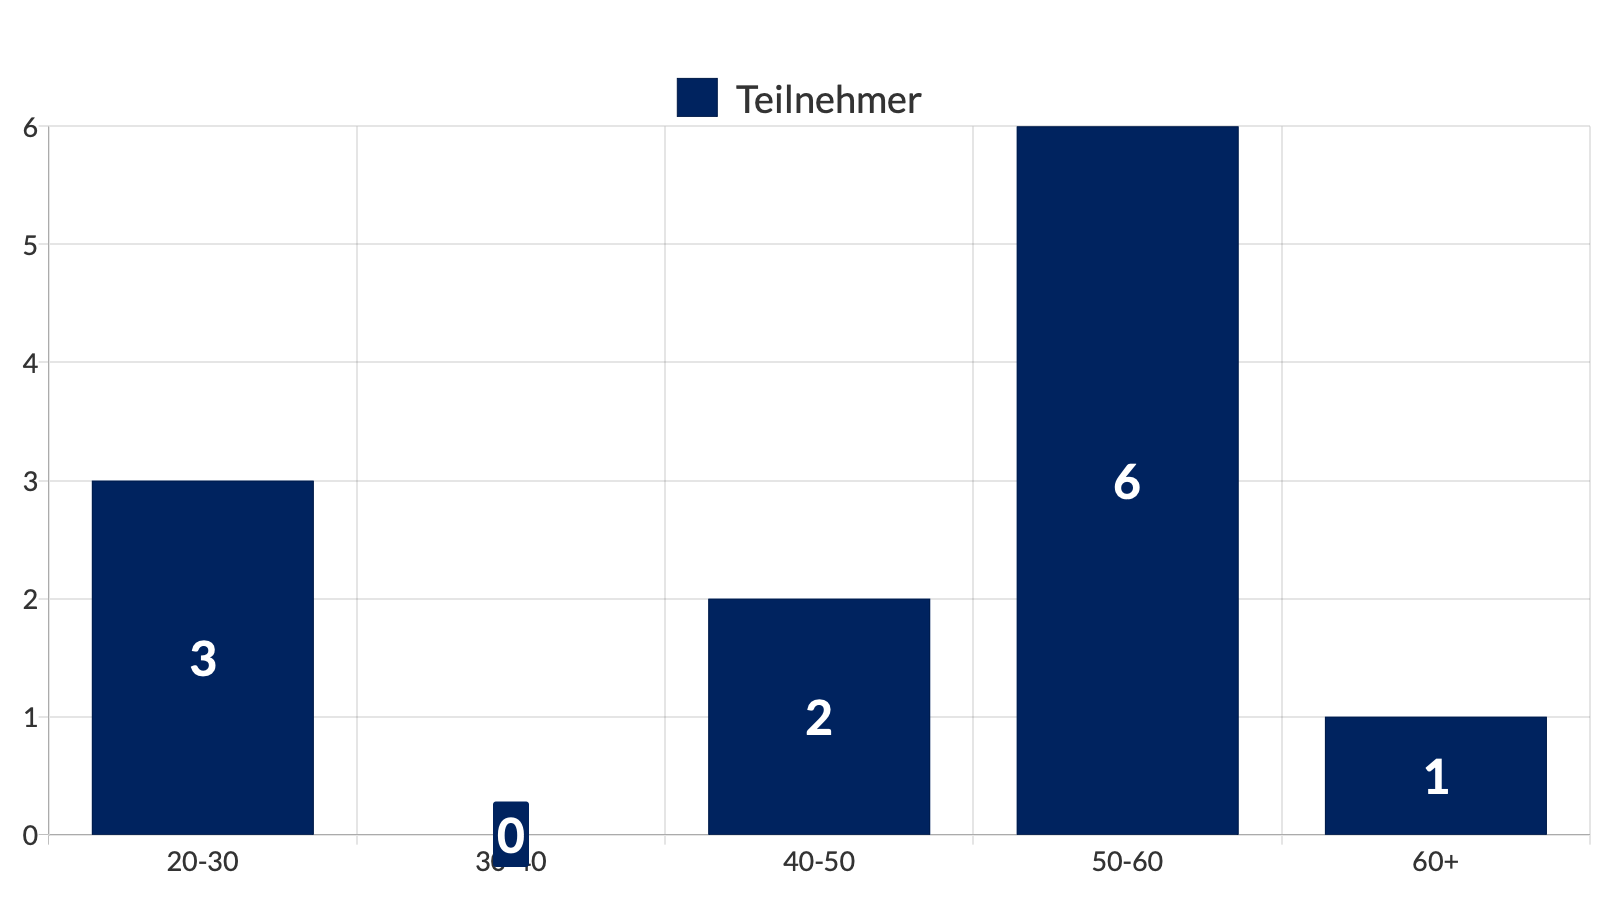
\includegraphics[width=0.8\textwidth]{img/abbildungen/chart-2.png}
	\captionsetup{format=hang}
	\caption{Alter der Teilnehmer}
\end{figure}

Dabei ist auffällig, dass die Teilnehmer der Befragung überwiegend der Gruppe 50-60 Jahre zugehörig sind. Auch die Gruppe 20-30 Jahre ist häufig vertreten. Lediglich die Gruppe 40-50 Jahre ist wenig vertreten. Daraus lässt sich schließen, dass die Teilnehmer der Befragung überwiegend entweder neu in das Berufsfeld eingestiegen sind oder bereits eine langjährige Erfahrung in diesem Bereich haben. 

Vor Beginn der Befragung wurden die Teilnehmer gebeten anzugeben, welche Rolle sie innerhalb des Teams einnehmen. Daraus lassen sich zwei Gruppen bilden: Development und Operations. Die Verteilung der Teilnehmer auf die beiden Gruppen ist in der folgenden Grafik dargestellt:

\begin{figure}[h]
	\centering 
	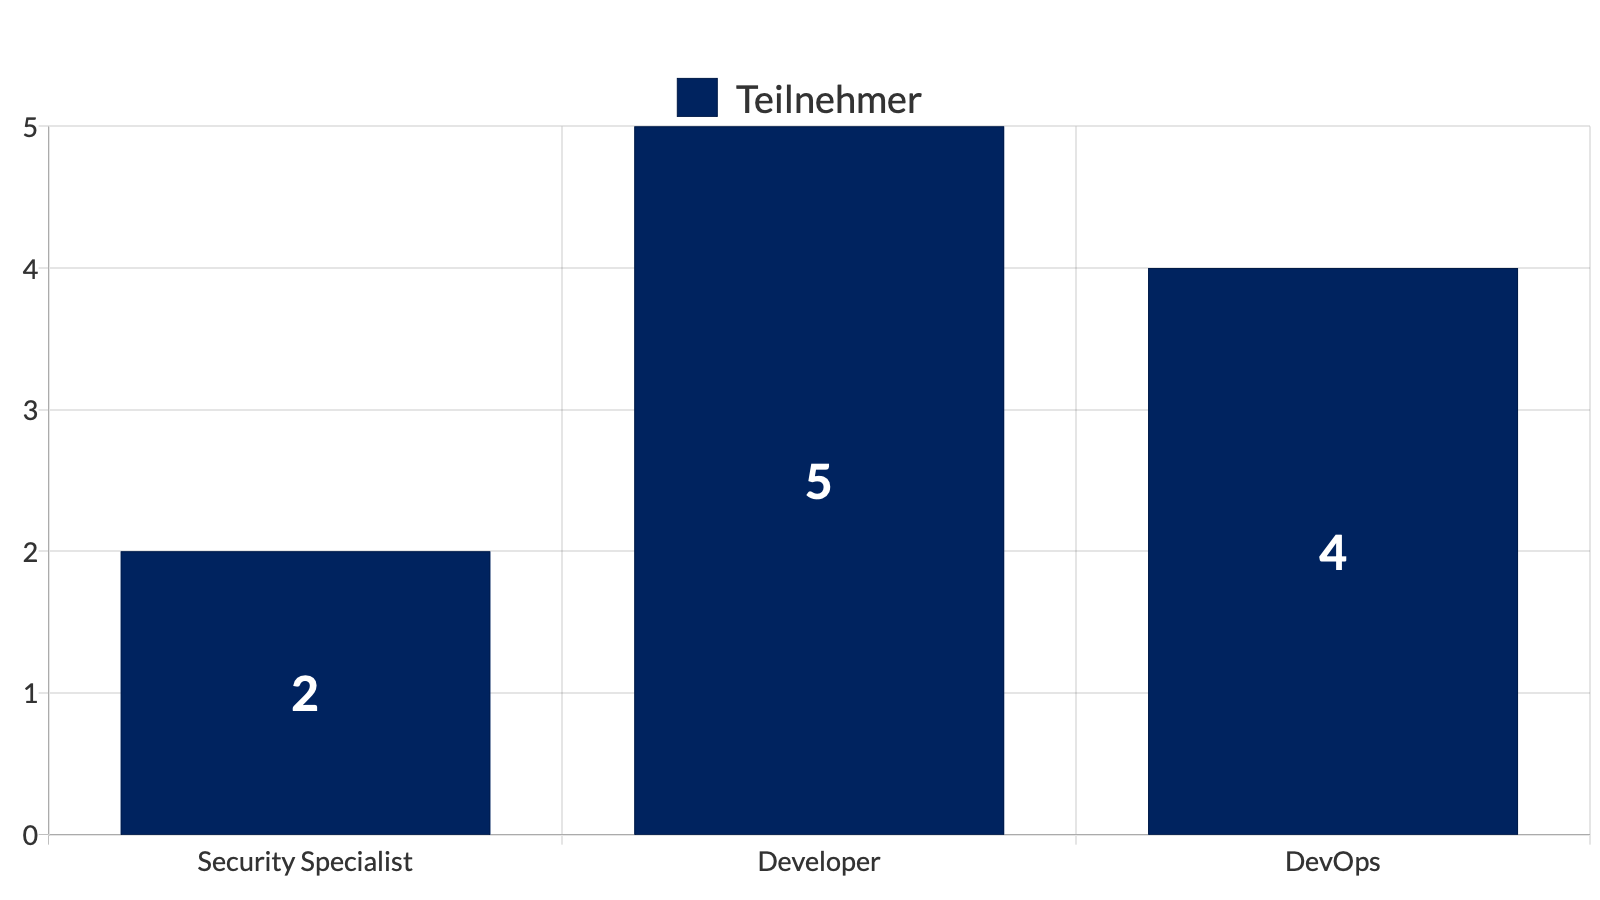
\includegraphics[width=0.7\textwidth]{img/abbildungen/chart_rollen.png}
	\captionsetup{format=hang}
	\caption{Alter der Teilnehmer}
\end{figure}

\subsection{Inhalt der Demonstration}
Allen Teilnehmern wurde vor der Befragung eine Live-Demonstration der Registrierung und Anmeldung mit Hilfe eines Security Keys gezeigt. Der Security Key wurde zu Beginn der Demonstration in einen üblichen USB-Slot eines Firmenlaptops eingesteckt und nach der Demonstration an die Teilnehmer übergeben. 

Die Anmeldung/Registrierung ist in mehrere Schritte unterteilt. Zunächst bestätigt der Nutzer, dass er sich mit Hilfe eines Security Keys anmelden/registrieren möchte:

\begin{figure}[h]
	\centering 
	
\includegraphics[width=0.7\textwidth]{img/abbildungen/reg001.png}
	\captionsetup{format=hang}
	\caption{Veränderter Keycloak-Login}
\end{figure}

Darauf folgt ein Dialogfeld des Browsers, welcher den Nutzer dazu auffordert zu bestätigen, dass der Security Key registriert wird. Dieser Schritt ist einmalig und findet nur bei der Registrierung statt. Ist der Security Key bereits registriert, wird dieser Schritt übersprungen:

\begin{figure}[h]
	\centering 
	
\includegraphics[width=0.7\textwidth]{img/abbildungen/reg002.png}
	\captionsetup{format=hang}
	\caption{Veränderter Keycloak-Login}
\end{figure}

Nach der Bestätigung des Dialogs muss der Nutzer den PIN des Security Keys eingeben:

\begin{figure}[H]
	\centering 
	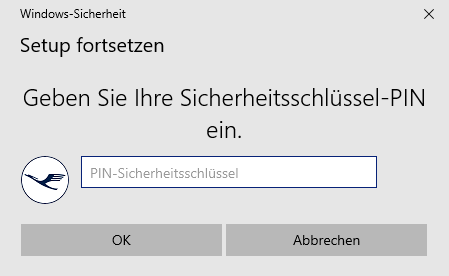
\includegraphics[width=0.7\textwidth]{img/abbildungen/reg003.png}
	\captionsetup{format=hang}
	\caption{Veränderter Keycloak-Login}
\end{figure}

Ist die richtige PIN eingegeben wurden, erscheint ein letztes Fenster, welches den Nutzer dazu auffordert den Knopf des Security Keys zu drücken. Erst danach ist der Browser dazu autorisert sich mit Hilfe des Security Keys gegen den Keycloak-Server zu registrieren oder anzumelden:

\begin{figure}[h]
	\centering 
	
\includegraphics[width=0.7\textwidth]{img/abbildungen/reg004.png}
	\captionsetup{format=hang}
	\caption{Veränderter Keycloak-Login}
\end{figure}

Sobald der Knopfdruck erfolgt, wird der Nutzer erfolgreich eingeloggt. Diese Informationen wurden den Teilnehmern ebenfalls während der Durchführung des Fragebogens mitgeteilt. 

Nachdem die Registrierung und Anmeldung mit Hilfe eines Security Keys demonstriert wurde, wurde den Teilnehmern ebenfalls eine mögliche Anmeldung mit Hilfe eines Passkeys gezeigt. Der Prozess beginnt ebenfalls bei Abbildung xy und hat lediglich einen Folgeschritt:

\begin{figure}[h]
	\centering 
	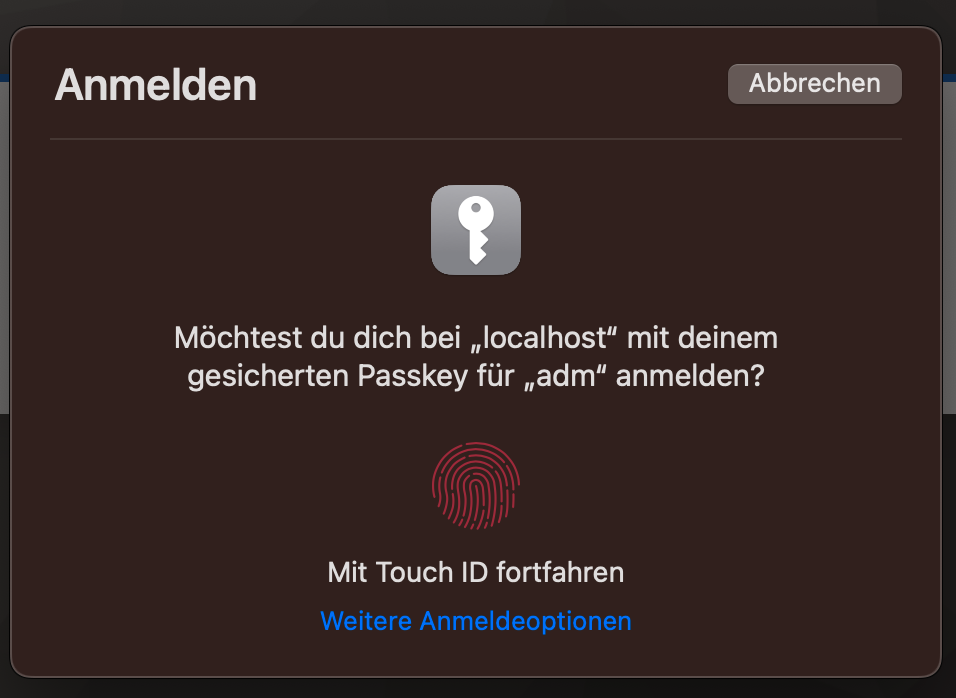
\includegraphics[width=0.7\textwidth]{img/abbildungen/passkey_demo.png}
	\captionsetup{format=hang}
	\caption{Veränderter Keycloak-Login}
\end{figure}

Für die Demonstration wurde hierbei ein privates Gerät genutzt (Apple Macbook Air M1), welches mit einem Touch ID Scanner ausgestattet ist.


\subsection{Herleitung der Fragen} \label{questions}
Aufgrund des Ziels der Befragung, eine Aussage über die Akzeptanz und die Benutzerfreundlichkeit einer passwortlosen Authentifizierung zu treffen, werden lediglich Fragen gestellt, die sich auf diese beiden Punkte beziehen. Um eine hohe Teilnahme zu gewährleisten, werden die Fragen möglichst kurz gehalten und nur wenige Fragen gestellt. Die Fragen werden so gestaltet, dass sie dem Teilnehmer die Möglichkeit bietet Kommentare zu hinterlassen oder seine Antwort zu begründen. Die Fragen werden so gestellt, dass sie einfach zu verstehen sind und kein Vorkenntnisse im Bereich der passwortlosen Authentifizierung voraussetzen. Im folgenden werden die Fragen begründet aufgelistet und erläutert:

\paragraph{Frage 1:}

\begin{quote}
    \textit{Hast du schonmal einen Security Key genutzt?}
\end{quote}
\textbf{Antwörtmöglichkeiten:} Ja; Nein; 

Diese Frage leitet sich aus \cite{farke2020you} ab. Die Antwortmöglichkeiten werden im Vergleich aber angepasst und reduziert. Durch die Reduzierung auf zwei Antwortmöglichkeiten wird eine bessere Auswertung ermöglicht. Antworten Teilnehmer mit \textit{Ja}, werden sie gefragt in welchem Kontext sie den Security Key genutzt haben. So lassen sich zusätzliche Informationen über die Nutzungsdauer und den Zweck der Nutzung zu erhalten.

\paragraph{Frage 2:}

\begin{quote}
    \textit{Bist du generell bereit deine Passwörter durch eine andere Art der Authentifizierung zu ersetzen?}
\end{quote}
\textbf{Antwörtmöglichkeiten:} Ja; Nein; 

Diese Frage ergibt sich aus einer Umfrage von Statista, in welcher Teilnehmer gefragt wurden, durch welche Art der Authentifizierung sie das Passwort ersetzen würden. Lediglich 22\% der Teilnehmer gaben an, dass sie ihr Passwort lieber beibehalten würden \cite{techstat}. Daraus folgt die Annahme, dass eine Vielzahl an Nutzern grundsätzlich dazu bereit wären ihr Passwort zu ersetzen. Die Frage soll eine bessere Analyse der folgenden Fragen ermöglichen und zielt auf die Akzeptanz einer passwortlosen Authentifizierung im generellen ab.

\paragraph{Frage 3:}

\begin{quote}
    \textit{Benutzt du auf der Arbeit aktuell einen Passwort Manager?}
\end{quote}

\textbf{Antwörtmöglichkeiten:} Ja; Nein;

Verwandte Studien zeigen, dass Nutzer eines Passwort Managers teilweise eine geringere Anmeldezeit auf Grund eines Passwort Managers aufweisen (insbesondere bei einer Nutzung von autofill) \cite{farke2020you}. Die Frage soll einen Zusammenhang zwischen der Nutzung eines Passwort Managers und der Einschätzung der Benutzerfreundlichkeit einer passwortlosen Authentifizierung ermöglichen.

\paragraph{Frage 4:}

\begin{quote}
    \textit{Kennst du das FIDO2-Protokoll und weißt du grob wie es funktioniert?}
\end{quote}

\textbf{Antwörtmöglichkeiten:} Ja; Nein;

Diese Frage bezieht sich auf die in Kapitel xy aufgeführte Problematik, dass Nutzer lieber Passwörter nutzen, da sie die Funktionsweise und Technologie im Hintergrund besser verstehen \cite{lyastani2020fido}. Dieser mögliche Zusammenhang soll betrachtet werden. Antworten Teilnehmer mit \textit{Ja}, werden sie gefragt, ob sie die Funktionsweise des FIDO2-Protokolls erklären können. So lässt sich eine Aussage über die Kenntnisse der Teilnehmer treffen. 

\paragraph{Frage 5:}

\begin{quote}
    \textit{Wie bewertest du die Benutzerfreundlichkeit der Registrierung mit Hilfe eines Security Keys?}
\end{quote}

\textbf{Antwörtmöglichkeiten:} Besser als mit einem Passwort; Gleich gut wie mit einem Passwort; Schlechter als mit einem Passwort;

Diese Frage soll einen Vergleich zwischen der Benutzerfreundlichkeit einer passwortlosen Authentifizierung und einer passwortbasierten Authentifizierung ermöglichen. Aus diesem Grund wurden die Antwortmöglichkeiten bewusst so gewählt, dass sie einen Vergleich ermöglichen. Eine generelle Bewertung würde die Auswertung erschweren, da die Teilnehmer unterschiedliche Vergleichswerte wählen könnten.

\paragraph{Frage 6:}

\begin{quote}
    \textit{Wie bewertest du die Benutzerfreundlichkeit der Anmeldung mit Hilfe eines Security Keys?}
\end{quote}

\textbf{Antwörtmöglichkeiten:} Besser als mit einem Passwort und \ac{MFA}; Gleich gut wie mit einem Passwort und \ac{MFA}; Schlechter als mit einem Passwort und \ac{MFA};

Wie auch Frage fünf zielt diese Frage auf die Benutzerfreundlichkeit ab. Die Unterteilung in zwei Fragen ergibt sich vor allem aus der Tatsache, dass sich die Registrierung und die Anmeldung, insbesondere bei einer passwortbasierten Authentifizierung, deutlich unterscheiden. Während es sich bei einer Anmeldung lediglich um eine Wissensabfrage handelt, muss bei der Registrierung zunächst ein eigenes Passwort erstellt werden. Dies könnte dazu führen, dass die beiden Abläufe unterschiedlich bewertet werden und somit der Vergleich zur passwortlosen Authentifizierung erschwert wird.

\paragraph{Frage 7:}

\begin{quote}
    \textit{Wärst du dazu bereit einen Security Key für den privaten Gebrauch zu kaufen, wenn der Preis bei ca. 50€ liegt?}
\end{quote}

\textbf{Antwörtmöglichkeiten:} Ja; Nein;

Diese Frage zielt auf die Akzeptanz einer passwortlosen Authentifizierung im privaten Kontext ab und basiert auf dem Ergebnis aus Kapitel xy. Dort wurde festegestellt, dass der Kaufpreis eines Security Keys ebenfalls eine Hürde für die Nutzung darstellen kann. Als Richtwert für den Kaufpreis wird hierbei der ungefähre Preis eines Yubikeys der Series 5 mit NFC gewählt, da dieser ebenfalls für die Umsetzung genutzt wird. Die Frage soll im Weiteren auch auf für die Nutzung im Unternehmenskontext genutzt werden, da die Akzeptanz im Generellen auch eine Auswirkung auf die Etablierung von Security Keys hat. Eine erhöhte Etablierung kann ebenfalls zu einer breiteren Unterstüzung führen.

\paragraph{Frage 8:}

\begin{quote}
    \textit{Hältst du einen Security Key für sicherer als ein Passwort?}
\end{quote}

\textbf{Antwörtmöglichkeiten:} Ja; Nein;

Diese Frage basiert auf der in Kapitel xy beschriebenen Annahme, dass Nutzer an der Sicherheit von Security Keys zweifeln, da sie die Funktionsweise der Technologie nicht verstehen. Dies soll im Zusammenhang mit Frage 4 betrachtet werden. Bewusst wird dabei auf die Antwortmöglichkeit \textit{Ich weiß es nicht} verzichtet, da Teilnehmer auf der Basis ihres aktuellen Wissensstands eine intuitive Entscheidung treffen sollen. Dies ermöglicht ebenfalls eine Aussage über die Akzeptanz der Teilnehmer. 

\paragraph{Frage 9:}

\begin{quote}
    \textit{Findest du eine Anmeldung per Passkey besser als eine Anmeldung per Security Key?}
\end{quote}

\textbf{Antwörtmöglichkeiten:} Ja; Nein; Gleich;

Diese Frage soll für einen Ausblick genutzt werden, ob eine Anmeldung per Passkey eine Alternative zu einer Anmeldung per Security Key darstellt. In \textbf{\ref{fido2-pros}} wurde ebenfalls deutlich, dass die Benutzerfreundlichkeit weniger von \ac{FIDO}2 abhängig ist, sondern viel mehr vom genutzten authentifizerungsgerät.  Mit Hilfe von kommentaren der Teilnehmer sollen konkrete Vor- und Nachteile der beiden Verfahren in Bezug auf deren Benutzerfreundlichkleit ermittelt werden.


\subsection{Auswertung}
Die Auswertung der Fragebögen bestätigt in vielen Teilen die bereits erarbeiteten Annahmen aus Kapitel xy. Lediglich zwei der Teilnehmer geben an, dass sie bereits einen Security Key genutzt haben. Dies allerdings nur testweise und nicht im alltäglichen Gebrauch. Die restlichen Teilnehmer geben an, dass sie noch keinen Security Key genutzt haben bzw. lediglich einen gesehen haben. Dies bestätigt, dass die Nutzung von Security Keys aktuell noch nicht weit verbreitet ist und Passwörter weiterhin die dominierende Methode der Authentifizierung darstellen.

Alle Teilnehmer geben an, dass sie dazu bereit wären ihr Passwort durch eine andere Art der Authentifizierung zu ersetzen. Dies übertrifft das Ergebnis aus \cite{techstat}. Dies kann daran liegen, dass alle Teilnehmer in einem sehr technischen Kontext arbeiten und somit eine höhere Akzeptanz für neue Technologien aufweisen und ein höheres Bewusstsein für Sicherheit innerhalb der Informatik aufweisen. 

\begin{figure}[H]
	\centering 
	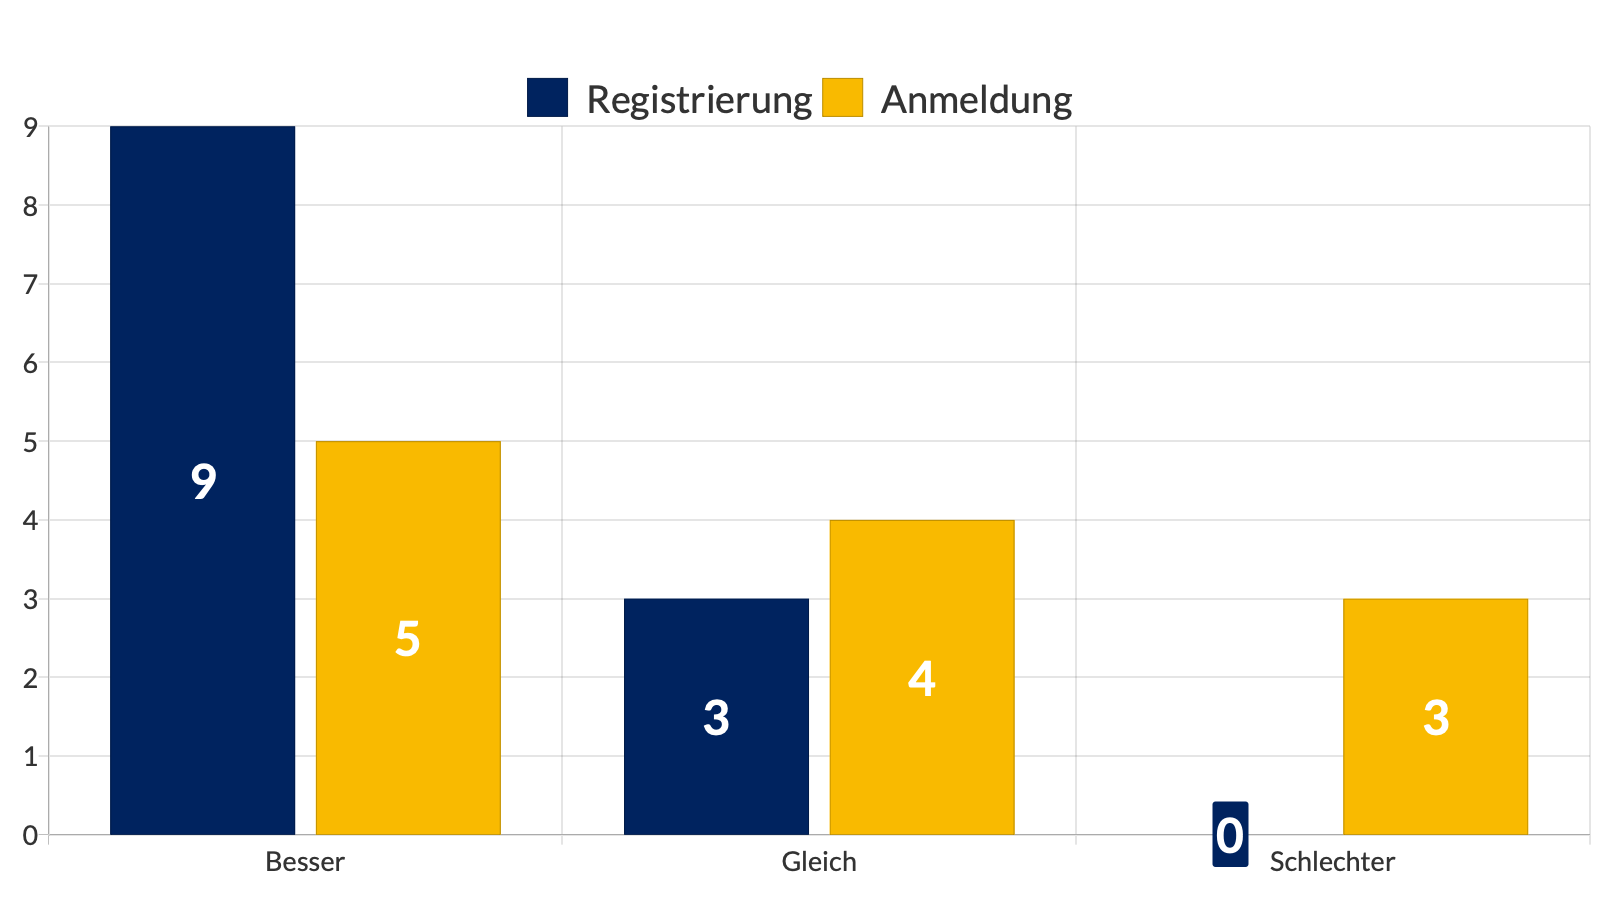
\includegraphics[width=0.7\textwidth]{img/abbildungen/chart_anmeldung_register.png}
	\captionsetup{format=hang}
	\caption{Veränderter Keycloak-Login}
\end{figure}

Bei der Bewertung der Registrierung und der Anmeldung mit Hilfe eine Security Keys sind deutliche Unterschiede sichtbar. Die deutliche Mehrheit der Teilnehmer bevorzugte die Registrierung per Security Key gegenüber der passwortbasierten Alternative. Keiner der Teilnehmer fand die Registrierung im Vergleich schlechter. Bei der Anmeldung hingegen ist ein ausgeglicheneres Ergebnis sichtbar. Im Vergleich geben drei der Teilnehmer an, dass sie Anmeldung schlechter finden als die aktuelle Alternative mit Hilfe eines Passwortes und \ac{MFA}. Es wird also deutlich, dass die beiden Abläufe der Registrierung und der Anmeldung differenziert betrachtet werden müssen. 
Eine Abhängigheit zwischen der Nutzung eines Passwort Managers und der Bewertung der Benutzerfreundlichkeit lässt sich nicht feststellen, da lediglich drei Teilnehmer keinen Passwort Manager nutzen und diese sehr verschiedene Bewertungen abgeben. Eine aussagekräftige Auswertung ist somit nicht möglich. 


Zehn der Teilnehmen geben an, dass sie nicht bereit wären 50€ für einen Security Key auszugeben. Dies bestätigt die Annahme aus Kapitel xy, dass der Preis eine Hürde für die Nutzung und Etablierung darstellen kann. Eine vermehrte Nutzung im privaten Kontext würde zu mehr Akzeptanz führen, da die Teilnehmer bereits mit der Technologie vertraut sind. 

Bis auf zwei Teilnehmer wird die Nutzung von Security Keys sicherer eingeschätzt als die Nutzung von Passwörtern. Da lediglich zwei Nutzer die Nutzung als weniger sicher betrachten lässt sich keine Aussage über einen Zusammenhang zwischen der Kenntnis des FIDO2-Protokolls und der Einschätzung der Sicherheit treffen.

Zwölf der Teilnehmer geben an eine Anmeldung per Passkey besser zu finden als eine Anmeldung per Security Key. 

Aus den Kommentaren lassen sich ebenfalls einige Erkenntnisse ziehen:

\begin{itemize}
    \item Ein Teilnehmer stufte die Registrierung und ANmeldung als \glqq\textit{sehr aufregend}\grqq, da es etwas neues ist und begründete so seine positive Bewertung. Dieses Beispiel zeigt auf, dass die Gewöhnung an eine neue Technologie nicht zwangsweise negativ ist, sondern auch positiv bewertet werden kann.
    \item Mehrere Teilnehmer kritisierten die Notwendigkeit den Security Key immer dabei haben zu müssen und spontane Logins nicht möglich sind. Dies deckt sich mit den Ergebnissen aus Kapitel xy.
    \item Daraus resultiere auch der Kritikpunkt, dass zusätzliche Hardware verloren gehen kann. Dies ist ein weiterer Kritikpunkt, welcher bereits in Kapitel xy aufgeführt wurde.
    \item Mehrere Teilnehmer wiesen darauf hin, dass sie ihr Handy und somit ihre Authenticator App im dabei haben. Selbst, wenn sie den Prozess des anmeldens mit Hilfe eines Security Keys als besser bewerten, würden sie weiterhin die Nutzung eines Passwortes mit \ac{MFA} bevorzugen. 
    \item Ein neuer Punkt der in den Kommentaren aufgeführt wurde ist, dass \ac{SSO} ein wichtiger Faktor ist. Da somit eine geringere Abfrage der Passwörter gegeben ist und auch weniger Passwörter erstellt werden müssen. Dies wirkt sich auch auf die EInschätzung der Benutzerfreundlichkeit aus.
    \item Die Mehrheit der Teilnehmer war der Meinung, dass sie die Benutzerfreundlichkeit der Security Keys erst nach einer längeren Testphase bewerten können.
    \item Ein Kritikpunkt der Teilnehmer am Anmeldevorgang mit Hilfe eines Security Keys ist, dass die EIngabe der PIN und des Benutzernamens zu viel sind. Dadurch bewerteten sie die Alternative als gleich oder schlechter als die aktuelle Lösung. Sie wünschen sich eine Lösung, bei dem der Security Key lediglich eingesteckt und gedrückt werden muss.
    \item Ein Teilnehmer begründete seine Antwort bezogen auf die Passkeys damit, dass er zusätzliche Hardware für sicherer hält und sich bei der Nutzung von Passkeys nicht sicher ist, ob diese wirklich nur auf dem Gerät gespeichert werden.
    \item Einige Teilnehmer erläuterten, dass sie die Anmeldung per Security Key benutzerfreundlicher als ein Passwort mit \ac{MFA} finden, allerdings nicht besser als lediglich einem Passwort.
    \item Ebenfalls wurde die mechanische Belastung des Security Keys und des USB-Ports genannt. Beide könnten durch die Nutzung beschädigt werden. Auch dieser Punkt wurde bereits in Kapitel xy aufgeführt.
    \item Auch der Preis wurde häufig als Kritikpunkt genannt. Ergänzend erwähnte allerdings ein Teilnehmer, dass er den Preis bezahlen würde, wenn es weiter etabliert ist. Ein anderer Teilnehmer erwähnte, dass er zum aktuellen Zeitpunkt maximal 20€ für einen Security Key ausgeben würde.
    \item Zur reinen Benutzerfreundlichkeit merkte ein Teilnehmer an, dass ein schlechtes und einfach gewähltes Passwort deutlich benutzerfreundlicher sei, wenn man den Faktor der Sicherheit nicht betrachtet.
\end{itemize}

\subsection{Fazit \& Reflexion}
Aus der Auswertung der Kommentare lässt sich ebenfalls eine Reflexion des Fragebogens ableiten. Ein entscheidenes Feedback ist dabei, die Testphase zu verlängern. Da der Bearbeitungszeitraum dieser Arbeit begrenzt ist und zunächst eine Implementierung erfolgen musste war dies nicht möglich. Aus diesem Grund wurde lediglich dieser Fragebogen erstellt, um einen ersten Eindruck zu erhalten. Für eine weitere Ausarbeitung sollte allerdings eine längere Testphase eingeplant werden. 


\section{Wirtschaftlichkeit}
Ein entscheidender Faktor für den Einsatz einer passwortlosen Authentifizierung mit Hilfe eines Security Keys ist die Wirtschaftlichkeit. Im Folgenden soll eine Analyse der Wirtschaftlichkeit im Bezug auf die Abteilung cGroup Solutions durchgeführt werden.

Betrachtet man die Teamgröße von 15 Personen und geht von den aktuellen Kosten eines Yubikeys aus (50€) so ergibt sich ein Gesamtpreis von 750€. Dieser Preis ist einmalig und muss nicht wiederholt werden. Auf Grund der geringen Backup-Möglichkeiten eines Security Keys sollte allerdings ein Backup-Key pro Nutzer angeschafft werden. Dieser kann im Falle eines Verlustes des ersten Keys genutzt werden. Dies erhöht die Kosten auf 1500€.
Lässt man alternativ weiterhin eine Anmeldung per Passwort zu, würden 750€ entfallen, allerdings wäre der eigentliche Zweck der Anschaffung nicht mehr erfüllt.
Sollte ein Security Key verloren oder kaputt gehen muss dieser ebenfalls ersetzt werden.
Zusätzlich zu den Materialkosten müssen die Kosten für die Implementierung betrachtet werden. Die Migration von Passwörtern auf Security Keys muss von erfahrenen Entwicklern und Architekten durchgeführt werden. Die genauen Kosten dafür lassen sich allerdings nicht definieren und sind stark abhängig von der gewünschten Implementierung. 

Sollte eine Anschaffung für das gesamte Unternehmen \ac{LSY} erfolgen so würde sich der Preis auf 280.000€ belaufen. Dies ergibt sich aus der aktuellen Mitarbeiterzahl von 2.800€ und den Kosten eines Security Keys von 50€, sowie einem Backup-Key pro Nutzer.

Im Gegenzug muss ein möglicher Kostenvorteil eingerechnet werden. Da Passwörter wie in Kapitel xy beschrieben eine der größten Schwachstellen darstellen, sind sie ein grundlegender Faktor für erfolgreiche Angriffe. Würde eine Nutzung der Security Keys dies verhindern oder eindämmen, so würde dies zu einer Kostenreduktion führen. Auch hier lassen sich allerdings nur schwierig konkrete Zahlen nennen. Diese sind unter anderem abhängig von der Schwere und Art des Angriffs. Einen Richtwert liefert der \textit{Cost of a Data Breach Report 2023} von IBM \cite{databreach}. Dort werden die durchschnittlichen Kosten eines Data Breach für bestimmte Regionen aufgezählt. Der Wert für die Region Deutschland liegt bei 4,67 Millionen US-Dollar \cite{databreach}. Daraus lässt sich folgern, dass ein erfolgreicher Angriff auf die \ac{LSY} zu einem deutlich höheren Kostenaufwand führen kann, als die Anschaffung von Security Keys.



\chapter{Fazit \& Empfehlung}
Das Fazit der Arbeit lässt sich in drei Teile Aspekte gliedern. Diese leiten sich aus den Zielen der Arbeit ab, welche in \textbf{\ref{target}} definiert wurden. Es handelt sich dabei um die Aspekte der Sicherheit, der Benutzerfreundlichkeit und der Umsetzbarkeit im Bezug auf einer passwortlosen \ac{SFA}. Das gesamte Fazit dieser Arbeit bezieht sich dabei lediglich auf die passwortlose Authentifizierung mit FIDO2, da die anderen passwortlosen Verfahren nicht weiter betrachtet wurden.

\paragraph*{Sicherheit:} Grundsätzlich handelt es sich bei FIDO2 Protokoll an sich um eine deutlich sicherere Alternative zu einer passwortbasierten Authentifizierung. So übersteigt eine Nutzung von FIDO2 Zugangsdaten auch die Sicherheit einer Nutzung von Passwörtern inklusive \ac{MFA}. Dies liegt insbesondere an der Nutzung von geprüfter asymmetrischer Kryptografie. Es gibt keine geteilten Geheimnisse und der private Schlüssel wird nur lokal auf dem Gerät des Nutzers gespeichert. So werden die meisten Angriffsvektoren der klassischen Passwortauthentifizierung eliminiert. FIDO2 Zugangsdaten lassen sich nicht erraten, phishen und können nicht von Datenlecks betroffen sein. Zudem gilt CTAP2.1 in Verbindung mit WebAuthn als \ac{PQ} bereit. Es handelt sich also auch um eine zukunftsfähige Technologie. Dennoch besteht eine große Abhängigkeit zum genutzten Authentifizierungsgerät. Eine Nutzung von Security Keys führt zu physischen Angriffsvektoren. So kann dieser beispielsweise von Diebstahl betroffen sein. Allerdings lassen sich Security Keys meisten mit einer PIN oder einem biometrischen Merkmal absichern. Dennoch wird die Sicherheit im Vergleich zur passwortbasierten Alternative als höher eingestuft.

\paragraph*{Benutzerfreundlichkeit:} Wie auch im Aspekt der Sicherheit besteht hier eine große Abhängigkeit zum genutzten Authentifizierungsgerät. Grundsätzlich ist FIDO2 in Form von CTAP2.1 und WebAuthn bereits weitreichend verbreitet. Es wird von den meisten Browsern nativ unterstützt und auch Anbieter wie Apple, Microsoft und Google ermöglichen die Nutzung von FIDO2. Nutzer müssen sich keine Passwörter mehr ausdenken und sich diese merken, was einen großen Vorteil darstellt. Dennoch zeigt diese Arbeit auch einige Kritikpunkte auf - insbesondere im Bezug auf die Nutzung von Security Keys. Diese stellen für viele Nutzer eine große Hürde dar. Nutzer kritisierten den Security Key immer bei sich haben zu müssen. Das physische Objekt kann zudem verloren oder kaputt gehen. In solchen Fällen besteht ebenfalls oftmals kein effektiver und sicherer Proezess für eine Wiederherstellung des Zugangs. Auch der entstehende Kostenaufwand und die Verwaltung einer Vielzahl an Security Keys kann im Unternehmenskontext eine Hürde darstellen. Die meisten Nutzer sind zusätzlich so sehr an die Nutzung von Passwörtern gewöhnt, dass es Prozess der Umgewöhnung benötigt wird, um die Akzeptanz zu erhöhen.

\paragraph*{Umsetzbarkeit:} Die Umsetzbarkeit einer Integration von Security Keys mit Hilfe von FIDO2 innerhalb der \ac{LSY} stellt sich in dieser Arbeit als größte Hürde dar. Dies liegt insbesondere an der festen Verankerung der passwortbasierten Authentifizierung in das Sicherheitskonzept und die Richtlinien der \ac{LSY}. Diese zu verändern benötigt einen langen und aufwändigen Prozess. Auch auf technischer Ebene kann sich eine Umstellung in einem so großem Ausmaß als schwierig darstellen. Diese ist aber grundsätzlich möglich und wird von dem Großteil der Systeme unterstützt. Dennoch bestehen auch Sonderfälle, in welchen weiterhin eine Nutzung von Passwörtern notwendig ist. Trotz der weitreichen Unterstützung von FIDO2 ist diese nicht vergleichbar mit der Etablierung von Passwörtern. Dennoch zeigt die Testphase dieser Arbeit auch, dass eine Umstellung der Authentifizierung möglich ist und diese mit einem verhältnismäßig geringen Aufwand umgesetzt werden kann. Mit der aktuellen Umsetzung innerhalb der \ac{LSY} ist eine Nutzung von Security Keys lediglich für eine \ac{MFA} möglich. 

In Kapitel xy wurden insbesondere drei Ziele der Arbeit definiert. Diese werden im Folgenden bewertet. 
Die Ergebnisse der Arbeit machen deutlich, welche Schwachstellen und Angriffsvektoren aufzeigen. Aus diesem Grund existiert jedoch nicht bloß eine Alternative. Es gibt verschiedene passwortlose Ansätze, welche sich für verschiedene Anwendungsfälle eignen. Jeder Ansatz hat dabei seine Vor- und Nachteile. Deutlich wird jedoch, dass das FIDO2-Projekt zu den meist untestützten und am weitesten verbreiteten Ansätzen gehört. Dies liegt auch an der gebotenen Vielfalt, da FIDO2 nicht nur Security Keys, sondern beispielsweise auch Passkeys unterstützt.
Im Bezug auf Sicherheit ist das FIDO2-Protokoll eine erhebliche Verbesserung gegenüber der klassischen Passwortauthentifizierung. Da FIDO2 auf öffentliche/private Schlüssel basiert fallen die meisten Angriffsvektoren der klassischen Passwortauthentifizierung weg. 

Aus diesen Gründen empfiehlt sich die Integration von FIDO2 als Alternative ebenfalls für den Unternehmenskontext. Für die Nutzung von Security Keys hingegegen lässt sich keine eindeutige Empfehlung auf den gegebenen Kontext der \ac{LSY} aussprechen. Dies geht vor allem aus den Umsetzungsmöglichkeiten und der erarbeiteten Benutzerfreundlichkeit hervor. Aktuell ist eine FIDO2 Authentifizierung mit Hilfe eines Security Keys noch nicht ausreichend etabliert, um eine gesamte Umstellung vornehmen zu können. Nicht alle Dienste ermöglichen eine FIDO2 Authentifizierung. Zum aktuellen Zeitpunkt eignet sich die Nutzung von Security Keys lediglich für eine \ac{MFA}. Das Ergebnis dieser Arbeit ist allerdings, dass sich die Nutzung von Security Keys insbesondere für eine \ac{SFA} eignet.

Dies entspricht nicht den Richtlinien \ac{SFA}. Solange allerdings keine weitreichende Unterstützung von FIDO2 erfolgt, wird keine Änderung dieser Richtlinie empfohlen. Die Nutzung von Security Keys als zusätzlicher Faktor wird aus wirtschaftlichen Gründen nicht empfohlen. In diesem Fall ist die Nutzung einer Authenticator App besser geeignet.

Grundsätzlich ist eine Nutzung von FIDO2 als Alternative zur klassischen Passwortauthentifizierung zu empfehlen. Sobald eine ausschließliche Nutzung ermöglicht wird lassen siche erhebliche Vorteile für die Sicherheit erzielen. Lediglich die Nutzung von Security Keys ist nicht zweifelsfrei zu empfehlen. In dieser Arbeit werden mehrere Kritikpunkte an der Benutzerfreundlichkeit aufgezeigt. Fragwürdig ist, ob diese Kritikpunkte nach einer erweiterten Gewöhnungsphase noch bestehen. Eine Lösung könnte die Nutzung von Passkeys darstellen. Diese sind allerdings noch nicht weitreichend verbreitet.

Daraus folgt die Empfehlung für die \ac{LSY} nicht direkt auf FIDO2 in Kombination mit Security Keys zu setzen. Stattdessen sollte das Bewusstsein für passwortlose Alternativen erweitert werden. Die Offenheit für Alternativen sollte ebenfalls gefördert. Zusätzlich sollte die Etablierung von FIDO2 weiter beobachtet werden. Sobald eine ausschließliche Nutzung möglich ist, sollte eine Umstellung erfolgen.

\chapter{Ausblick Passkeys}
Ein Problem der Nutzung von FIDO2 mit Hilfe von Security Keys ist die Abhängigkeit an ein einzelnes Gerät. Mit Passkeys stellt FIDO2 eine Alternative, welche multi-device fähige Zugangsdaten ermöglicht \cite{usecasfido}.

Abhängigkeit von Anbietern für beispielsweise Authenticator Apps, welche diese Möglichkeit integrieren müssen. Technisch ist dies mit FIDO2 allerdings schon integriert \cite{usecasfido}.

Erhöhte Benutzerfreundlichkeit gegenüber Security Keys. Keine zusätzliche Hardware notwendig, bzw. möglich mehrere Geräte zu nutzen \cite{usecasfido}.

Vergleichbar wie die Nutzung von auto fill Passwortmanagern, allerdings mit erhöhter Sicherheit und ohne Notwendigkeit von \ac{MFA} \cite{usecasfido} \cite{passkeysgoogle}.

Typischerweise würde die für CTAP2.1 benötigte autorisierung mit Hilfe eines biometrisches Merkmales erfolgen \cite{usecasfido}.

So würde eine Abhängigkeit an die Hardware-Anbieter bestehen. Denn die Sicherheit der Passkeys würde von der Sicherheit der Hardware und des Betriebsystems abhängen, auf welchem die Passkeys gespeichert werden \cite{usecasfido}.

Zusätzlich ermöglicht der FIDO2 Standard die Nutzung von Bluetooth. Dies ermöglicht eine Nutzung von Passkeys mit mobilen Geräten. Dies ist eine Absicherung, falls eine Synchronisierung von Passkeys nicht möglich ist. Dies könnte beispielsweise der Fall sein, wenn Geräte unterschiedlicher Anbieter genutzt werden \cite{usecasfido}.

Dabei kann zusätzlich zum synchronisierten Passkey optional ein Gerätespezifischer Schlüssel erzeugt werden. Der Passkey kann somit nur mit den Geräten genutzt werden, welche einen Gerätespezifischen Schlüssel besitzen \cite{usecasfido}. Dies würde die Sicherheit erhöhen, da die Anbieter der Synchronisierungsdienste keinen Zugriff auf die Passkeys hätten.

Der Google Password Manager ermöglicht bereits eine Synchronisierung der Passkeys und verschlüsselt diese zusätzlich. Der benötigte private Schlüssel für die Verschlüssellung wird dabei lediglich auf dem Gerät selbst gespeichert und ist dort zusätzlich verschlüsselt \cite{passkeysgoogle}.

Zusätzlich ermöglicht dieser auch die Nutzung des Passkeys inklusive eines device-bound Schlüssels. Dieser Schlüssel wird auf Android Geräten auf der \ac{TEE} gespeichert. Somit ist dieser zusätzlich auf der Hardware-Ebene geschützt. Das bedeutet allerdings auch, dass dieser nicht von Backups betroffen ist und nicht wiederherstellbar ist \cite{passkeysgoogle}.

Auch Apple bietet die synchronisierte Nutzung von Passkeys an. Diese werden dabei in der iCloud Keychain gespeichert. Diese ist dabei ebenfalls lediglich in verschlüsselter Form synchronisiert. Eine Möglichkeit zur Nutzung von Passkeys inkluse eines device-bound Schlüssels wird aktuell nicht in der Dokumentation von Apple erwähnt \cite{passkeysapple}.

\begin{figure}[h]
	\centering 
	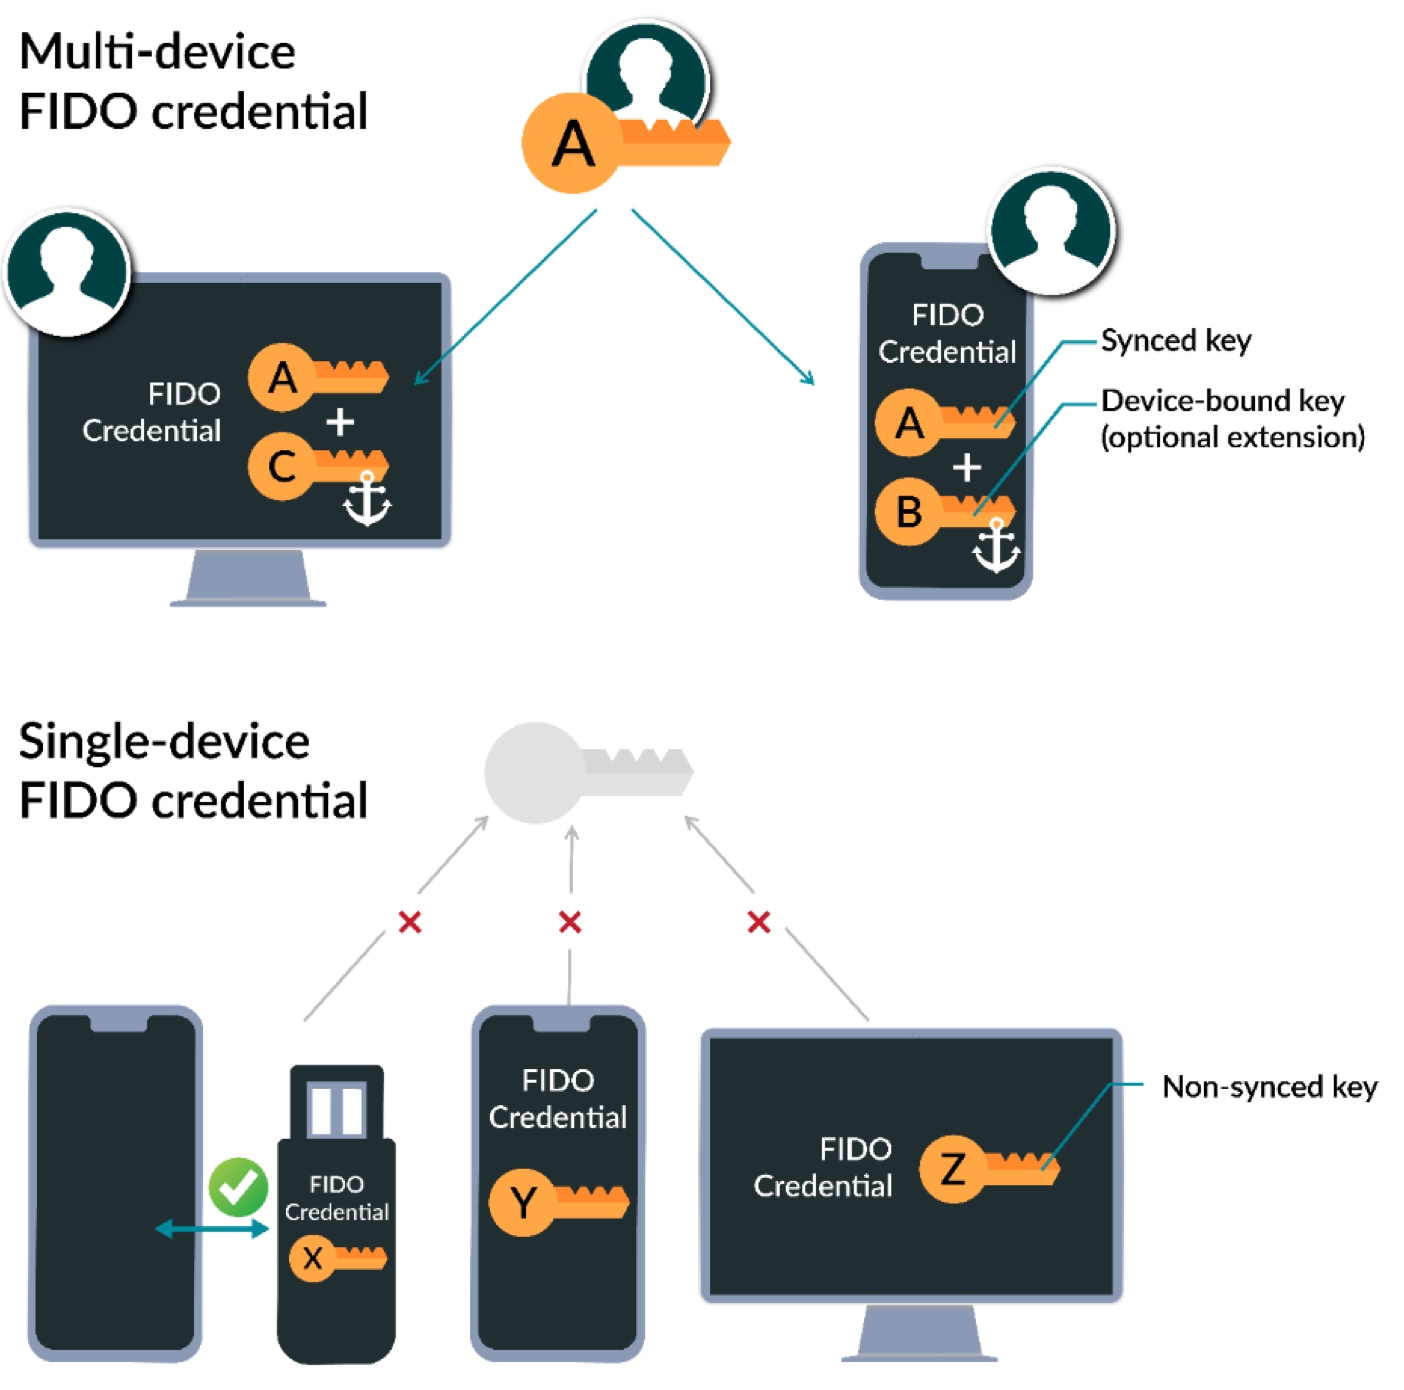
\includegraphics[width=0.7\textwidth]{img/abbildungen/multi-device-fido2.png}
	\captionsetup{format=hang}
	\caption{Multi-device FIDO und Single-device FIDO \cite{usecasfido}} \label{azure-seckey}
\end{figure}







\printbibliography[title=Literaturverzeichnis]
% Der Anhang beginnt hier - jedes Kapitel wird alphabetisch aufgezählt. (Anhang A, B usw.)
%\appendix
%\ihead{\appendixname~\thechapter} % Neue Header-Definition


% appendix.tex einziehen
%\chapter{Anhang}
\lipsum


\end{document}
